\documentclass{book}

\title{Analisi Matematica T-A}
\author{Michele Mazza}
\date{November 2023}


% Pacchetti di Codifica e Lingua
\usepackage[utf8]{inputenc}
\usepackage[T1]{fontenc}
\usepackage[italian]{babel}

% Pacchetti Grafici e Diagrammi
\usepackage{graphicx}
\usepackage{tikz}
\usepackage{tikz-3dplot}
\usetikzlibrary{angles,quotes,arrows.meta, positioning}
\usepackage{pgfplots}
\pgfplotsset{compat=1.18}

% Pacchetti Matematici
\usepackage{amsmath, amssymb, amsthm}

% Pacchetti per Tabelle e Unità di Misura
\usepackage{geometry}
\usepackage{siunitx}
\usepackage{booktabs}
\usepackage{tabularx}
\usepackage{colortbl}

% Pacchetti per Layout e Formattazione
\usepackage{fancyhdr}
\usepackage{float}
\usepackage{microtype}

% Altri Pacchetti Utili
\usepackage{mdframed}
\usepackage{animate}

% Pacchetto enumitem
\usepackage{enumitem}

% Definizioni dei Colori
\definecolor{lightblue}{HTML}{9cd8fc}
\definecolor{myblue}{HTML}{139FE9}

% Definizione del comando \norm
\newcommand{\norm}[1]{\left\lVert#1\right\rVert}

%\font\nullfont=cmr10 

% Ambienti Personalizzati
\newmdtheoremenv[
    backgroundcolor=orange!10,
    linecolor=myblue,
    linewidth=0pt,
    leftmargin=0pt,
    rightmargin=0pt,
    innerleftmargin=10pt,
    innerrightmargin=10pt,
    innertopmargin=10pt,
    innerbottommargin=10pt,
    nobreak
]{curiosity}{Curiosità}

\newmdtheoremenv[
    font=\normalfont\small,
    linewidth=0pt,
    innerleftmargin=10pt,
    innerrightmargin=10pt,
]{example}{Esempio}

\newmdtheoremenv[
  backgroundcolor=lightblue,
  linecolor=myblue,
  linewidth=1.5pt,
  innertopmargin=10pt,
  innerbottommargin=10pt,
  innerrightmargin=10pt,
  innerleftmargin=10pt,
  nobreak
]{theorem}{Teorema}

\newmdtheoremenv[
  backgroundcolor=gray!10,
  linewidth=0pt,
  innertopmargin=10pt,
  innerbottommargin=10pt,
  innerrightmargin=10pt,
  innerleftmargin=10pt,
  nobreak
]{definition}{Definizione}

\newmdtheoremenv[
  backgroundcolor=gray!10,
  linecolor=myblue,
  linewidth=1.5pt,
  innertopmargin=10pt,
  innerbottommargin=10pt,
  innerrightmargin=10pt,
  innerleftmargin=10pt,
  nobreak
]{proposition}{Proposizione}

% Configurazioni di fancyhdr
\pagestyle{fancy}
\fancyhf{} % Pulisce tutti i campi
\fancyhead[LE,RO]{\thepage} % Numero di pagina
\fancyhead[RE]{\nouppercase{\leftmark}} % Titolo del capitolo
\fancyhead[LO]{\nouppercase{\rightmark}} % Titolo della sezione
\renewcommand{\headrulewidth}{0.5pt}
\renewcommand{\footrulewidth}{0pt}

\geometry{a4paper, left=20mm, right=20mm, top=20mm, bottom=20mm}

% Pacchetto Hyperref (inserito per ultimo)
\usepackage{hyperref}

\begin{document}

\frontmatter
\maketitle
\tableofcontents
\mainmatter

\chapter{Funzioni}

\section{Definizioni}
\begin{definition}
    \subsection{Funzione}
    Siano \(X\) e \(Y\) due insiemi, una \textbf{funzione} \( f : X \rightarrow Y\) è una corrispondenza che associa ad ogni elemento \(x \in X\) uno e uno solo elemento \(y \in Y\)
\end{definition}
\begin{center}
    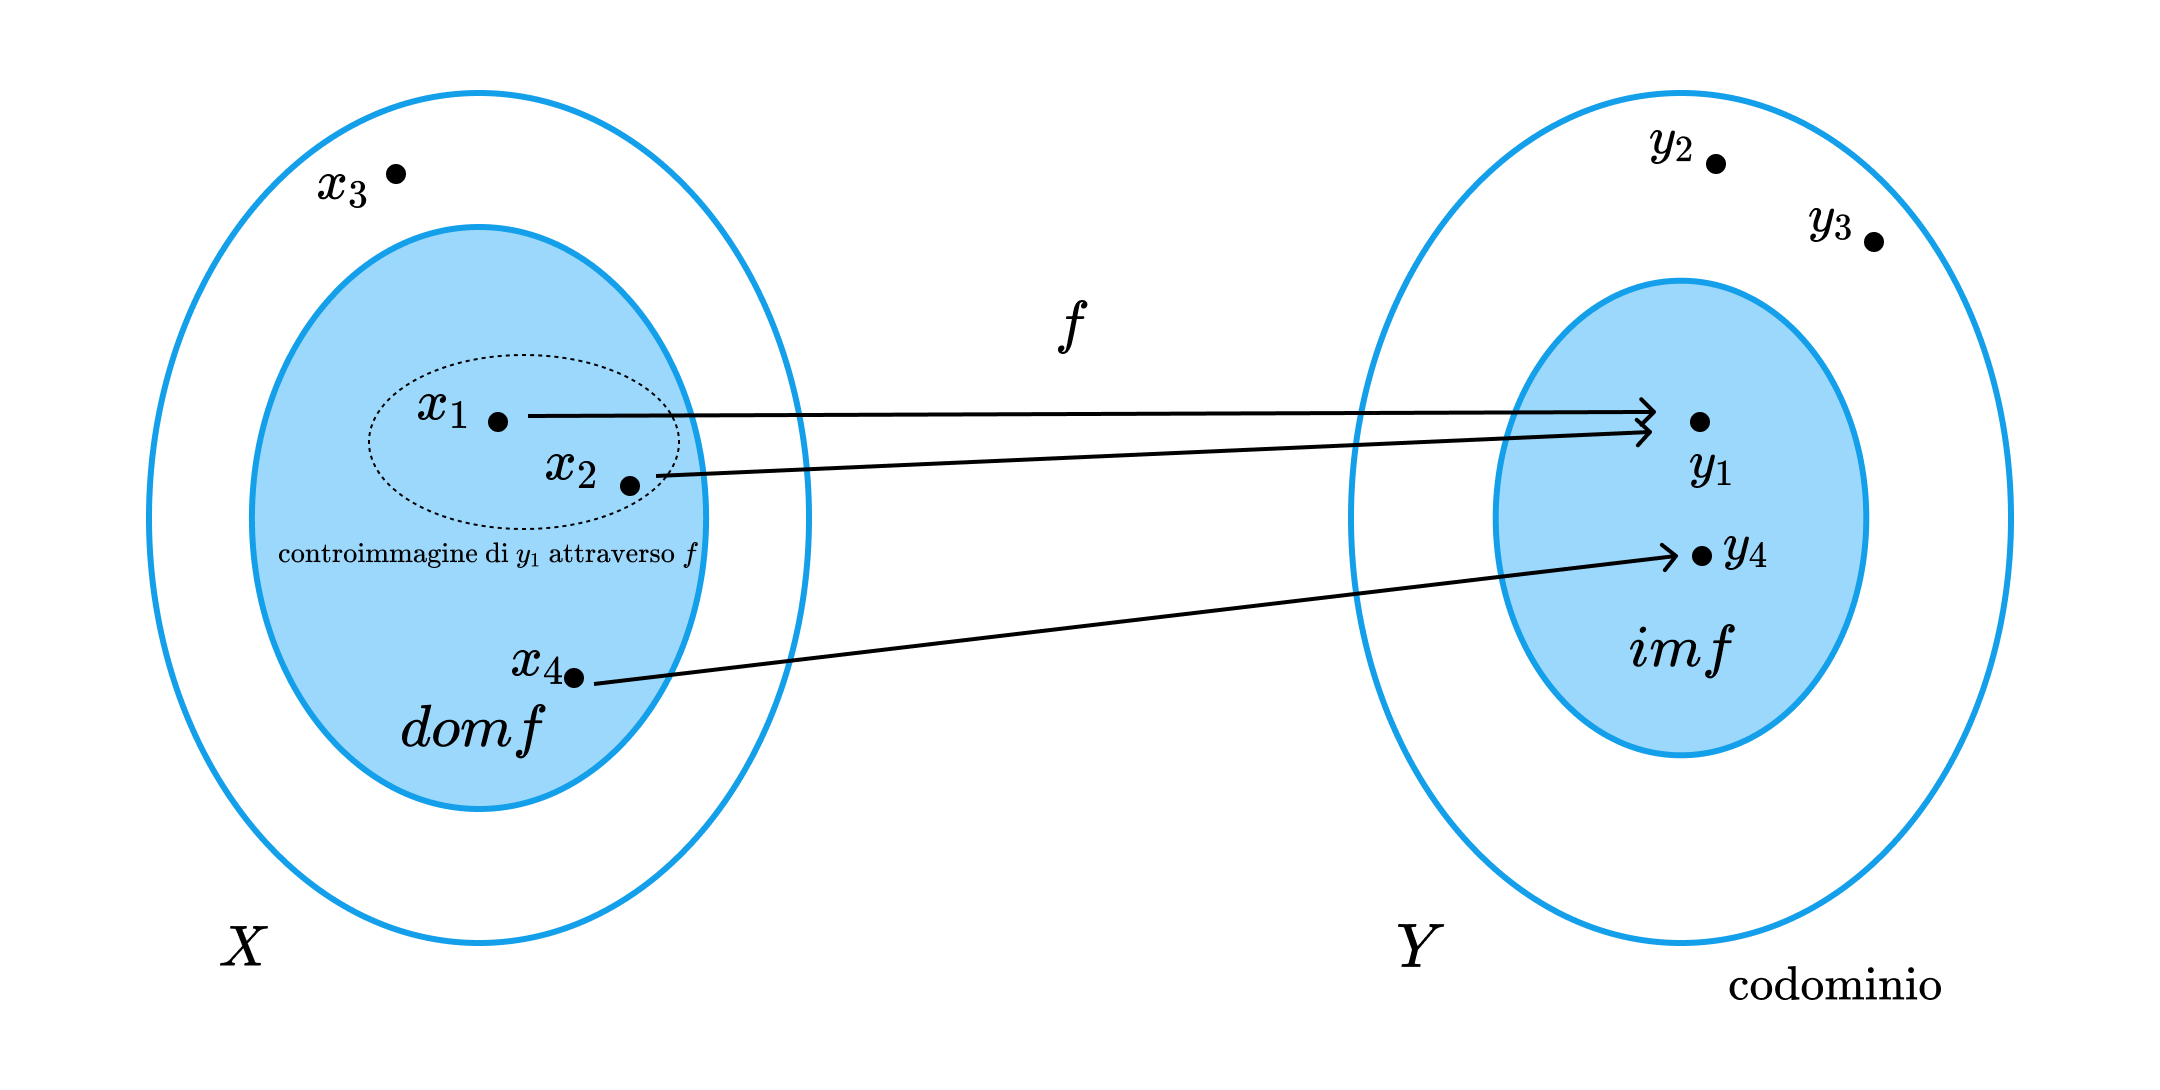
\includegraphics[width=0.8\textwidth]{source/00 funzione.png}
\end{center}

\begin{definition}
    \subsection{Dominio}
    Sia \( f: X \rightarrow Y \) una funzione. Il \textbf{dominio} di \( f \), indicato con \( \text{dom}(f) \), è l'insieme di tutti i valori di input per i quali la funzione \( f \) è definita. In termini formali,
    \[ \text{dom}(f) = X \]
    che è l'insieme da cui ogni \( x \) viene scelto per l'applicazione della funzione \( f \).
\end{definition}

\begin{definition}
    \subsection{Immagine}
    Sia \( f: X \rightarrow Y \) una funzione. L'\textbf{immagine} di \( f \), indicata con \( \text{im}(f) \), è l'insieme di tutti i valori che \( f \) può assumere come output. In termini formali,
    \[ \text{im}(f) = \{ f(x) \mid x \in X \} \]
    che è un sottoinsieme di \( Y \).
\end{definition}
\noindent\begin{minipage}{\textwidth}
    \begin{definition}
        \subsection{Codominio}
        Sia \( f: X \rightarrow Y \) una funzione. Il \textbf{codominio} di \( f \) è l'insieme \( Y \) stesso. Il codominio rappresenta tutti i possibili valori che \( f \) può teoricamente assumere come output, indipendentemente dal fatto che questi valori vengano effettivamente raggiunti o meno quando la funzione è applicata agli elementi di \( X \).

        Ad esempio, consideriamo la funzione \( f: \mathbb{R} \rightarrow \mathbb{R} \) definita da \( f(x) = x^2 \). Qui, il codominio è l'intero insieme dei numeri reali \( \mathbb{R} \), perché la funzione è definita in questo modo. Tuttavia, l'immagine di \( f \), cioè l'insieme dei valori che \( f \) effettivamente assume, è l'insieme dei numeri reali non negativi, poiché il quadrato di un numero reale non è mai negativo. Quindi, l'immagine è \( [0, \infty) \), un sottoinsieme del codominio \( \mathbb{R} \).
    \end{definition}
\end{minipage}

\begin{definition}
    \subsection{Controimmagine}
    Sia \( f: X \rightarrow Y \) una funzione e \( B \subseteq Y \) un sottoinsieme del codominio. La \textbf{controimmagine} (o pre-immagine) di \( B \) sotto \( f \), indicata con \( f^{-1}(B) \), è l'insieme di tutti gli elementi in \( X \) i cui valori sotto \( f \) appartengono a \( B \). In termini formali,
    \[ f^{-1}(B) = \{ x \in X \mid f(x) \in B \} \]
\end{definition}

\begin{example}
    \subsection{Esempi}
    Di seguito degli esempi di funzioni.
    \begin{enumerate}[label=\roman*., start=1]
        \item \noindent\begin{minipage}{\textwidth}
                  \(f : \mathbb{R} \rightarrow \mathbb{R}, f(x) = ax+ b\) (con a,b coefficienti reali), una \textbf{retta}
                  \begin{figure}[H]
                      \centering
                      \begin{tikzpicture}[scale = 1,
                              declare function={
                                      f(\x) = 2*\x - 2;
                                  }]
                          \begin{axis}
                              [
                                  xlabel={\( x \)},
                                  ylabel={\( f(x) \)},
                                  xmin=-10, xmax=10,
                                  ymin=-10, ymax=10,
                                  grid=both,
                                  axis lines=middle,
                                  axis line style=->,
                                  grid style={line width=.1pt, draw=gray!10},
                                  major grid style={line width=.2pt,draw=gray!50},
                                  minor tick num=3,
                                  enlargelimits={abs=0.5},
                                  xlabel style={at={(ticklabel* cs:1)}, anchor=north west},
                                  ylabel style={at={(ticklabel* cs:1)}, anchor=south west},
                                  samples=100,
                                  unbounded coords=jump,
                                  legend pos=south east
                              ]
                              \addplot[domain=-5:7, ultra thick, smooth, color=myblue]{f(x)};
                              \legend{\(f(x) = 2x - 2\)};
                          \end{axis}
                      \end{tikzpicture}
                      \caption{Grafico di \(f(x) = 2x - 2\)}
                  \end{figure}
              \end{minipage}
        \item \noindent\begin{minipage}{\textwidth}
                  \(f : \mathbb{R} \rightarrow \mathbb{R}, f(x) = x^2\), una \textbf{parabola}
                  \begin{figure}[H]
                      \centering
                      \begin{tikzpicture}[scale = 1,
                              declare function={
                                      f(\x) = \x^2;
                                  }]
                          \begin{axis}
                              [
                                  xlabel={\( x \)},
                                  ylabel={\( f(x) \)},
                                  xmin=-10, xmax=10,
                                  ymin=-10, ymax=10,
                                  grid=both,
                                  axis lines=middle,
                                  axis line style=->,
                                  grid style={line width=.1pt, draw=gray!10},
                                  major grid style={line width=.2pt,draw=gray!50},
                                  minor tick num=3,
                                  enlargelimits={abs=0.5},
                                  xlabel style={at={(ticklabel* cs:1)}, anchor=north west},
                                  ylabel style={at={(ticklabel* cs:1)}, anchor=south west},
                                  samples=100,
                                  unbounded coords=jump,
                                  legend pos=south east
                              ]
                              \addplot[domain=-5:5, ultra thick, smooth, color=myblue]{f(x)};
                              \legend{\(f(x) = x^2\)};
                          \end{axis}
                      \end{tikzpicture}
                      \caption{Grafico di \(f(x) = x^2\)}
                  \end{figure}
              \end{minipage}
        \item \noindent\begin{minipage}{\textwidth}
                  \(f : \mathbb{R}\setminus \{0\} \rightarrow \mathbb{R}, f(x) = \frac{1}{x}\), un'\textbf{iperbole} riferita agli asintoti
                  \begin{figure}[H]
                      \centering
                      \begin{tikzpicture}[scale = 1,
                              declare function={
                                      f(\x) = 1/\x;
                                  }]
                          \begin{axis}
                              [
                                  xlabel={\( x \)},
                                  ylabel={\( f(x) \)},
                                  xmin=-5, xmax=5,
                                  ymin=-5, ymax=5,
                                  grid=both,
                                  axis lines=middle,
                                  axis line style=->,
                                  grid style={line width=.1pt, draw=gray!10},
                                  major grid style={line width=.2pt,draw=gray!50},
                                  minor tick num=3,
                                  enlargelimits={abs=0.5},
                                  xlabel style={at={(ticklabel* cs:1)}, anchor=north west},
                                  ylabel style={at={(ticklabel* cs:1)}, anchor=south west},
                                  samples=100,
                                  unbounded coords=jump,
                                  legend pos=south east
                              ]
                              \addplot[domain=-6:-0.01, ultra thick, smooth, color=myblue]{f(x)};
                              \addplot[domain=0.01:6, ultra thick, smooth, color=myblue]{f(x)};
                              \legend{\(f(x) = \frac{1}{x}\)};
                          \end{axis}
                      \end{tikzpicture}
                      \caption{Grafico di \(f(x) = \frac{1}{x}\)}
                  \end{figure}
              \end{minipage}
        \item
              \noindent\begin{minipage}{\textwidth}
                  \(f : [0,3] \rightarrow \mathbb{R}\),
                  \(
                  f(x) =
                  \begin{cases}
                      3x    & \text{se } 0 \leq x \leq 1, \\
                      4 - x & \text{se } 1 < x \leq 2,    \\
                      x - 1 & \text{se } 2 < x \leq 3.
                  \end{cases}
                  \)
                  una funzione reale di variabile reale può essere \textbf{definita a tratti},
                  \begin{figure}[H]
                      \centering
                      \begin{tikzpicture}[scale = 1,
                              declare function={
                                      f(\x) = 3*\x;
                                      g(\x) = 4-\x;
                                      h(\x) = \x-1;
                                  }]
                          \begin{axis}
                              [
                                  xlabel={\( x \)},
                                  ylabel={\( f(x) \)},
                                  xmin=-4, xmax=4,
                                  ymin=-4, ymax=4,
                                  grid=both,
                                  axis lines=middle,
                                  axis line style=->,
                                  grid style={line width=.1pt, draw=gray!10},
                                  major grid style={line width=.2pt,draw=gray!50},
                                  minor tick num=3,
                                  enlargelimits={abs=0.5},
                                  xlabel style={at={(ticklabel* cs:1)}, anchor=north west},
                                  ylabel style={at={(ticklabel* cs:1)}, anchor=south west},
                                  samples=100,
                                  unbounded coords=jump,
                                  legend pos=south east
                              ]
                              \addplot[domain=0:1, ultra thick, smooth, color=myblue]{f(x)};
                              \addplot[domain=1:2, ultra thick, smooth, color=myblue]{g(x)};
                              \addplot[domain=2:3, ultra thick, smooth, color=myblue]{h(x)};
                              \filldraw [white] (2 , 1) circle (1.5pt);
                              \draw [myblue] (2 , 1) circle (1.5pt);
                              \filldraw [myblue] (2 , 2) circle (1.5pt);
                          \end{axis}
                      \end{tikzpicture}
                      \caption{Grafico di una funzione definita a tratti}
                  \end{figure}
              \end{minipage}
        \item \noindent\begin{minipage}{\textwidth}
                  \(f : \mathbb{R} \rightarrow \mathbb{R}, \space f(x) = |x| \)
                  \(
                  f(x) = |x| =
                  \begin{cases}
                      x  & \text{se } x \geq 0, \\
                      -x & \text{se } x < 0.
                  \end{cases}
                  \)
                  la funzione \textbf{Valore Assoluto}
                  \begin{figure}[H]
                      \centering
                      \begin{tikzpicture}[scale = 1,
                              declare function={
                                      f(\x) = -\x;
                                      g(\x) = \x;
                                  }]
                          \begin{axis}
                              [
                                  xlabel={\( x \)},
                                  ylabel={\( f(x) \)},
                                  xmin=-4, xmax=4,
                                  ymin=-4, ymax=4,
                                  grid=both,
                                  axis lines=middle,
                                  axis line style=->,
                                  grid style={line width=.1pt, draw=gray!10},
                                  major grid style={line width=.2pt,draw=gray!50},
                                  minor tick num=3,
                                  enlargelimits={abs=0.5},
                                  xlabel style={at={(ticklabel* cs:1)}, anchor=north west},
                                  ylabel style={at={(ticklabel* cs:1)}, anchor=south west},
                                  samples=100,
                                  unbounded coords=jump,
                                  legend pos=south east
                              ]
                              \addplot[domain=-5:0, ultra thick, smooth, color=myblue]{f(x)};
                              \addplot[domain=0:5, ultra thick, smooth, color=myblue]{g(x)};
                              \legend{\(f(x) = |x|\)};
                          \end{axis}
                      \end{tikzpicture}
                      \caption{Grafico di \(f(x) = |x|\)}
                  \end{figure}
              \end{minipage}
        \item
              \noindent\begin{minipage}{\textwidth}
                  \(f : \mathbb{R} \rightarrow \mathbb{Z}, \space f(x) = sign(x) \)
                  \(
                  f(x) = sign(x) =
                  \begin{cases}
                      +1 & \text{se } x > 0, \\
                      0  & \text{se }  x = 0 \\
                      -1 & \text{se} x < 0.
                  \end{cases}
                  \)
                  la funzione \textbf{Segno}
                  \begin{figure}[H]
                      \centering
                      \begin{tikzpicture}[scale = 1,
                              declare function={
                                      f(\x) = -1;
                                      g(\x) = 1;
                                  }]
                          \begin{axis}
                              [
                                  xlabel={\( x \)},
                                  ylabel={\( f(x) \)},
                                  xmin=-4, xmax=4,
                                  ymin=-4, ymax=4,
                                  grid=both,
                                  axis lines=middle,
                                  axis line style=->,
                                  grid style={line width=.1pt, draw=gray!10},
                                  major grid style={line width=.2pt,draw=gray!50},
                                  minor tick num=3,
                                  enlargelimits={abs=0.5},
                                  xlabel style={at={(ticklabel* cs:1)}, anchor=north west},
                                  ylabel style={at={(ticklabel* cs:1)}, anchor=south west},
                                  samples=100,
                                  unbounded coords=jump,
                                  legend pos=south east
                              ]
                              \addplot[domain=-5:0, ultra thick, smooth, color=myblue]{f(x)};
                              \addplot[domain=0:5, ultra thick, smooth, color=myblue]{g(x)};
                              \filldraw [myblue] (0 , 0) circle (1.5pt);
                              \filldraw [white] (0 , -1) circle (1.5pt);
                              \filldraw [white] (0 , 1) circle (1.5pt);
                              \draw [myblue] (0 , -1) circle (1.5pt);
                              \draw [myblue] (0 , 1) circle (1.5pt);
                              \legend{\(f(x) = sign(x)\)};
                          \end{axis}
                      \end{tikzpicture}
                      \caption{Grafico di \(f(x) = sign(x)\)}
                  \end{figure}
              \end{minipage}
        \item
              \noindent\begin{minipage}{\textwidth}
                  \(f : \mathbb{R} \rightarrow \mathbb{Z}, \space f(x) = [x] =\)  il più grande intero relativo \(\leq x\),  la funzione \textbf{Parte intera}
                  \begin{figure}[H]
                      \centering
                      \begin{tikzpicture}[scale = 1,
                              declare function={
                                      f(\x) = -2;
                                      g(\x) = -1;
                                      h(\x) = 0;
                                      i(\x) = 1;
                                      j(\x) = 2;
                                  }]
                          \begin{axis}
                              [
                                  xlabel={\( x \)},
                                  ylabel={\( f(x) \)},
                                  xmin=-2, xmax=2,
                                  ymin=-2, ymax=2,
                                  grid=both,
                                  axis lines=middle,
                                  axis line style=->,
                                  grid style={line width=.1pt, draw=gray!10},
                                  major grid style={line width=.2pt,draw=gray!50},
                                  minor tick num=3,
                                  enlargelimits={abs=0.5},
                                  xlabel style={at={(ticklabel* cs:1)}, anchor=north west},
                                  ylabel style={at={(ticklabel* cs:1)}, anchor=south west},
                                  samples=100,
                                  unbounded coords=jump,
                                  legend pos=south east
                              ]
                              \addplot[domain=-2:-1, ultra thick, smooth, color=myblue]{f(x)};
                              \addplot[domain=-1:0, ultra thick, smooth, color=myblue]{g(x)};
                              \addplot[domain=0:1, ultra thick, smooth, color=myblue]{h(x)};
                              \addplot[domain=1:2, ultra thick, smooth, color=myblue]{i(x)};
                              \addplot[domain=2:3, ultra thick, smooth, color=myblue]{j(x)};
                              \filldraw [white] (-2 , -2) circle (1.5pt);
                              \filldraw [white] (-1, -1) circle (1.5pt);
                              \filldraw [white] (0 , 0) circle (1.5pt);
                              \filldraw [white] (1 , 1) circle (1.5pt);
                              \filldraw [white] (2 , 2) circle (1.5pt);
                              \draw [myblue] (-2 , -2) circle (1.5pt);
                              \draw [myblue] (-1 , -1) circle (1.5pt);
                              \draw [myblue] (0 , 0) circle (1.5pt);
                              \draw [myblue] (1 , 1) circle (1.5pt);
                              \draw [myblue] (2 , 2) circle (1.5pt);
                              \filldraw [myblue] (-1 , -2) circle (1.5pt);
                              \filldraw [myblue] (0 , -1) circle (1.5pt);
                              \filldraw [myblue] (1 , 0) circle (1.5pt);
                              \filldraw [myblue] (2 , 1) circle (1.5pt);
                              \legend{\(f(x) = [x]\)};
                          \end{axis}
                      \end{tikzpicture}
                      \caption{Grafico di \(f(x) = [x]\)}
                  \end{figure}
              \end{minipage}
    \end{enumerate}
\end{example}
\newpage
\section{Funzioni iniettive, suriettive, biiettive}
Le tre proprietà che definiremo hanno un immediato riscontro grafico
nel caso di funzioni \(f\) reali di variabile reale. Precisamente, considerando il
grafico di \(f\) nel piano e le sue intersezioni con la famiglia di rette orizzontali,
la funzione risulta
\begin{enumerate}
    \item \textbf{iniettiva} se lo interseca al massimo in un punto,
    \item \textbf{suriettiva} su \(\mathbb{R}\) se ogni retta interseca il grafico in almeno un punto,
    \item \textbf{biiettiva} da \(\mathbb{R} \rightarrow \mathbb{R}\) se lo interseca esattamente in uno e un solo punto
\end{enumerate}
\noindent\begin{minipage}{\textwidth}
    \begin{definition}
        \subsection{Funzione iniettiva}
        Sia \(f:A \rightarrow B\). La funzione \(f\) è detta iniettiva se, per ogni coppia di elementi \(a_1, a_2 \in A\), \(a_1 \neq a_2\) \(\Rightarrow\) \(f(a_1) \neq f(a_2)\).
    \end{definition}
    \begin{figure}[H]
        \centering
        \begin{tikzpicture}
            \begin{axis}[
                    xlabel={\( x \)},
                    ylabel={\( f(x) \)},
                    xmin=-2, xmax=2,
                    ymin=-2, ymax=2,
                    grid=both,
                    axis lines=middle,
                    axis line style=->,
                    grid style={line width=.1pt, draw=gray!10},
                    major grid style={line width=.2pt,draw=gray!50},
                    minor tick num=5,
                    enlargelimits={abs=0.5},
                    ticklabel style={font=\small},
                    xlabel style={at={(ticklabel* cs:1)}, anchor=north west},
                    ylabel style={at={(ticklabel* cs:1)}, anchor=south west},
                    legend pos=south east
                ]
                \addplot[domain=-3:3, ultra thick, smooth, color=myblue] {x};
                \legend{Iniettiva}
            \end{axis}
        \end{tikzpicture}
        \begin{tikzpicture}
            \begin{axis}[
                    xlabel={\( x \)},
                    ylabel={\( f(x) \)},
                    xmin=-2, xmax=2,
                    ymin=-2, ymax=2,
                    grid=both,
                    axis lines=middle,
                    axis line style=->,
                    grid style={line width=.1pt, draw=gray!10},
                    major grid style={line width=.2pt,draw=gray!50},
                    minor tick num=5,
                    enlargelimits={abs=0.5},
                    ticklabel style={font=\small},
                    xlabel style={at={(ticklabel* cs:1)}, anchor=north west},
                    ylabel style={at={(ticklabel* cs:1)}, anchor=south west},
                    legend pos=south east
                ]
                \addplot[domain=-2:2, ultra thick, smooth, color=myblue] {x^2};
                \coordinate (A) at (axis cs:-1,1);
                \coordinate (B) at (axis cs:1,1);
                \coordinate (C) at (axis cs:-1,0);
                \coordinate (D) at (axis cs:1,0);
                \node at (A)[left] {$f(a_1)$};
                \node at (B)[right] {$f(a_2)$};
                \node at (C)[below left] {$a_1$};
                \node at (D)[below right] {$a_2$};
                \draw [dashed,thick](A) -- (B);
                \draw [dashed,thick](A) -- (C);
                \draw [dashed,thick](B) -- (D);
                \legend{Non iniettiva};
            \end{axis}
        \end{tikzpicture}
        \caption{Confronto tra una \(f(x)=x\) iniettiva, e \(f(x)=x^2\) non iniettiva}
    \end{figure}
\end{minipage}
\noindent\begin{minipage}{\textwidth}
    \begin{definition}
        \subsection{Funzione suriettiva}
        Sia \(f:A \rightarrow B\), se
        \[\ \forall\ b \in B, \exists\ f(a)=b\]
        allora f è suriettiva.
    \end{definition}
    \begin{figure}[H]
        \centering
        \begin{tikzpicture}
            \begin{axis}[
                    xlabel={\( x \)},
                    ylabel={\( f(x) \)},
                    xmin=-2, xmax=2,
                    ymin=-2, ymax=2,
                    grid=both,
                    axis lines=middle,
                    axis line style=->,
                    grid style={line width=.1pt, draw=gray!10},
                    major grid style={line width=.2pt,draw=gray!50},
                    minor tick num=5,
                    enlargelimits={abs=0.5},
                    ticklabel style={font=\small},
                    xlabel style={at={(ticklabel* cs:1)}, anchor=north west},
                    ylabel style={at={(ticklabel* cs:1)}, anchor=south west},
                    legend pos=south east
                ]
                \addplot[domain=-3:3, ultra thick, smooth, color=myblue] {x};
                \legend{Suriettiva}
            \end{axis}
        \end{tikzpicture}
        \begin{tikzpicture}
            \begin{axis}[
                    xlabel={\( x \)},
                    ylabel={\( f(x) \)},
                    xmin=-2, xmax=2,
                    ymin=-2, ymax=2,
                    grid=both,
                    axis lines=middle,
                    axis line style=->,
                    grid style={line width=.1pt, draw=gray!10},
                    major grid style={line width=.2pt,draw=gray!50},
                    minor tick num=5,
                    enlargelimits={abs=0.5},
                    ticklabel style={font=\small},
                    xlabel style={at={(ticklabel* cs:1)}, anchor=north west},
                    ylabel style={at={(ticklabel* cs:1)}, anchor=south west},
                    legend pos=south east
                ]
                \addplot[domain=-2:2, ultra thick, smooth, color=myblue] {x^2};
                \coordinate (A) at (axis cs:-3,0);
                \coordinate (B) at (axis cs:+3,0);
                \coordinate (C) at (axis cs:3,-3);
                \coordinate (D) at (axis cs:-3,-3);
                \fill[myblue, opacity=0.5] (A) -- (B) -- (C) -- (D) -- cycle;
                \legend{Non suriettiva};
            \end{axis}
        \end{tikzpicture}
        \caption{Confronto tra una \(f(x)=x\) suriettiva, e \(f(x)=x^2\) non suriettiva}
    \end{figure}
\end{minipage}
\begin{definition}
    \subsection{Funzione biunivoca}
    Sia \(f:A \rightarrow B\), se \(f\) è sia iniettiva che suriettiva, allora f è biiettiva(o biunivoca).
\end{definition}
\section{Funzione inversa}

La nozione di funzione inversa è centrale nell'analisi matematica e nelle sue applicazioni. Data una funzione \( f: A \rightarrow B \), l'inversa di \( f \), denotata come \( f^{-1} \), è una funzione da \( B \) a \( A \) tale che per ogni \( y \) nell'immagine di \( f \), \( f^{-1}(y) \) restituisce l'unico \( x \) in \( A \) per cui \( f(x) = y \).

\subsection{Condizioni per l'Invertibilità}
Una funzione deve essere iniettiva per avere un'inversa. L'iniettività garantisce che ogni elemento dell'immagine di \( f \) è associato a un unico elemento del dominio. Questa unicità è essenziale per definire \( f^{-1} \).

\subsection{Calcolo della Funzione Inversa}
Calcolare l'inversa di una funzione può essere un processo complesso. Per le funzioni algebriche, il metodo standard consiste nel risolvere l'equazione \( y = f(x) \) rispetto a \( x \). Questo approccio funziona bene per molte funzioni semplici. Tuttavia, esistono funzioni iniettive le cui inverse non possono essere espresse in forma chiusa. Una forma chiusa è un'espressione matematica finita che utilizza un numero finito di operazioni algebriche standard e funzioni elementari. Alcune funzioni iniettive, pur essendo teoricamente invertibili, non hanno un'espressione inversa semplice e diretta in termini di funzioni e operazioni elementari.


\subsection{Grafico della Funzione Inversa}
Il grafico di \( f^{-1} \) può essere ottenuto dal grafico di \( f \) scambiando gli assi \( x \) e \( y \). Questo scambio è equivalente a riflettere il grafico di \( f \) rispetto alla linea \( y = x \).
\begin{example}
    Prendo \[f :\ \mathbb{R} \rightarrow \mathbb{R},\ f(x) = x^2\]
    non è iniettiva.\\
    Prendo una \textbf{restrizione} \(A\) del dominio di \(f\), \(A=[0,+\infty)\) per renderla iniettiva.
    \[f|_{A}: [0,+\infty) \rightarrow \mathbb{R}, f(x) = x^2\]
    tale funzione è iniettiva e dunque invertibile e l'inversa è
    \[f|_{A}: [0,+\infty) \rightarrow \mathbb{R}, x = f^{-1}(y) = +\sqrt{y}\]
    Si preferisce effettuare il cambio di notazioni
    \[f|_{A}: [0,+\infty) \rightarrow \mathbb{R}, y = f^{-1}(x) = +\sqrt{x}\]
    \begin{figure}[H]
        \centering
        \begin{tikzpicture}
            \begin{axis}[
                    xlabel={\( x \)},
                    ylabel={\( f(x) \)},
                    xmin=0, xmax=2,
                    ymin=0, ymax=2,
                    grid=both,
                    axis lines=middle,
                    axis line style=->,
                    grid style={line width=.1pt, draw=gray!10},
                    major grid style={line width=.2pt,draw=gray!50},
                    minor tick num=5,
                    enlargelimits={abs=0.5},
                    xlabel style={at={(ticklabel* cs:1)}, anchor=north west},
                    ylabel style={at={(ticklabel* cs:1)}, anchor=south west},
                    samples=100,
                    unbounded coords=jump, % Gestisce i punti non definiti
                    legend pos=south east
                ]
                \addplot[domain=0:2, ultra thick, smooth, color=gray] {x^2};
                \addplot[domain=-0.5:3, thick, dashed, color=black] {x};
                \addplot[domain=0:3, ultra thick, smooth, color=myblue] {sqrt(x)};
                \legend{$y=x^2$, $y=x$, $y=+\sqrt{x}$};
            \end{axis}
        \end{tikzpicture}
    \end{figure}
\end{example}
\subsection{Ambiguità nella notazione e nel calcolo}
\begin{itemize}
    \item La notazione \( f^{-1} \) per la funzione inversa può portare a confusione, in particolare per chi si avvicina per la prima volta allo studio delle funzioni inverse. A differenza dell'inverso moltiplicativo, dove \( a^{-1} \) rappresenta l'elemento che, moltiplicato per \( a \), dà come risultato l'elemento neutro della moltiplicazione (tipicamente 1), la notazione \( f^{-1} \) non implica un'operazione aritmetica di inversione. Piuttosto, indica una funzione tale che, per ogni elemento \( y \) nell'immagine di \( f \), \( f^{-1}(y) \) restituisce l'elemento \( x \) del dominio di \( f \) per cui \( f(x) = y \).
    \item Un'altra fonte di ambiguità è il calcolo effettivo dell'espressione analitica di \( f^{-1} \). Per alcune funzioni, trovare la forma chiusa della funzione inversa è relativamente semplice e diretto, come nel caso delle funzioni lineari. Tuttavia, per altre funzioni, in particolare quelle non lineari o quelle che coinvolgono operazioni complesse, determinare \( f^{-1} \) in una forma esplicita può essere estremamente difficile, se non impossibile. Questo è dovuto al fatto che l'operazione di "invertire" una funzione non segue un processo standard e può richiedere metodi matematici avanzati o, in alcuni casi, può non avere una soluzione in termini di funzioni elementari.
    \item Inoltre, quando si riesce a trovare una formula per \( f^{-1} \), \textbf{spesso si effettua un cambio di variabili} per comodità. Inizialmente, se abbiamo \( x = f^{-1}(y) \), si può preferire riscrivere questa relazione come \( y = f^{-1}(x) \), scambiando semplicemente i simboli delle variabili. Questo non solo aiuta a mantenere una consistenza nella notazione, ma facilita anche il confronto e la rappresentazione grafica di \( f \) e \( f^{-1} \) sullo stesso sistema di coordinate. Un esempio di questo può essere visto nella transizione da una rappresentazione grafica a un'altra, come illustrato nella Figura 2.7 del testo, dove si passa da un grafico della funzione originale \( f \) a quello della sua inversa \( f^{-1} \).

\end{itemize}
\subsection{Esempi e Applicazioni}
\begin{itemize}
    \item \textbf{Funzione Logaritmica:} L'inversa della funzione esponenziale \( e^x \) è il logaritmo naturale \( \ln(x) \).
    \item \textbf{Funzioni Trigonometriche:} Le funzioni trigonometriche hanno inverse note come funzioni arcotrigonometriche, ma queste sono definite solo su intervalli specifici per mantenere l'iniettività.
\end{itemize}

\section{Funzioni monot\'one}
\begin{definition}
    \subsection{Funzione Monotona Crescente}
    Una funzione \( f \) si dice \textbf{monotona crescente} su un intervallo \( I \) se, per qualsiasi coppia di elementi \( x_1 \) e \( x_2 \) in \( I \) tali che \( x_1 < x_2 \), risulta sempre che \( f(x_1) \leq f(x_2) \). In forma simbolica, questo si esprime come:
    \[ \forall x_1, x_2 \in I, x_1 < x_2 \Rightarrow f(x_1) \leq f(x_2). \]

    Inoltre, la funzione \( f \) si dice \textbf{monotona strettamente crescente} su \( I \) se, per ogni coppia di elementi \( x_1 \) e \( x_2 \) in \( I \) con \( x_1 < x_2 \), si ha che \( f(x_1) < f(x_2) \). Questa condizione si può scrivere come:
    \[ \forall x_1, x_2 \in I, x_1 < x_2 \Rightarrow f(x_1) < f(x_2). \]
\end{definition}
\begin{figure}[H]
    \centering
    \begin{tikzpicture}
        \begin{axis}[
                xlabel={\( x \)},
                ylabel={\( y \)},
                xmin=0, xmax=2,
                ymin=0, ymax=2,
                grid=both,
                axis lines=middle,
                axis line style=->,
                grid style={line width=.1pt, draw=gray!10},
                major grid style={line width=.2pt,draw=gray!50},
                minor tick num=5,
                enlargelimits={abs=0.5},
                ticklabel style={font=\small},
                xlabel style={at={(ticklabel* cs:1)}, anchor=north west},
                ylabel style={at={(ticklabel* cs:1)}, anchor=south west},
                legend pos=south east
            ]
            \coordinate (A) at (axis cs:0.5,0.25);
            \coordinate (B) at (axis cs:1,1);
            \coordinate (Ay) at (axis cs:0,0.25);
            \coordinate (Ax) at (axis cs:0.5,0);
            \coordinate (By) at (axis cs:0,1);
            \coordinate (Bx) at (axis cs:1,0);
            \draw [dashed,thick](A) -- (Ay);
            \draw [dashed,thick](A) -- (Ax);
            \draw [dashed,thick](B) -- (Bx);
            \draw [dashed,thick](B) -- (By);
            \addplot[myblue, ultra thick, smooth, domain=0:2] {x^2};
            \filldraw [myblue] (A) circle (1.5pt);
            \filldraw [myblue] (B) circle (1.5pt);
            \legend{$y=x^2$};
        \end{axis}
    \end{tikzpicture}
    \caption{Funzione strettamente crescente su un intervallo I}
\end{figure}
\begin{proposition}
    Se \(f\) è strettamente monotona sul suo dominio, allora \(f\) è iniettiva.
\end{proposition}

\section{Funzioni composte}
\begin{definition}
    \subsection{Funzione Composta}
    Siano \( X \), \( Y \) e \( Z \) tre insiemi distinti. Sia \( f \) una funzione definita da \( X \) a \( Y \), e sia \( g \) una funzione definita da \( Y \) a \( Z \). Possiamo costruire una nuova funzione \( h \) definita da \( X \) a \( Z \) come la composizione di \( f \) e \( g \). Questa nuova funzione \( h \) è definita ponendo per ogni \( x \in X \):
    \[ h(x) = g(f(x)) \]
    \[h = g \circ f\]
\end{definition}

\section{Trasformazioni geometriche}
\begin{definition}
    \subsection{Traslazione di funzione mediante vettore(a,b)}
    Di seguito le traslazioni dato un vettore
    \( \vec{v} = (a,b)\text{, con }a>0, b>0 \)
    Ricordo che la traslazione di un punto di ottiene mediante
    \[T=\begin{cases}
            x_T=x+a \\
            y_T=y+b
        \end{cases}\]
    Mentre la traslazione di una funzione di ottiene mediante
    \[T^{-1}=\begin{cases}
            x_T=x-a \\
            y_T=y-b
        \end{cases}\]
\end{definition}
\subsubsection{Traslazione di vettore parallelo all’asse y (a=0,b=2).}
\[T^{-1}=\begin{cases}
        x_T=x-0 \\
        y_T=y-2
    \end{cases}\]
\begin{align*}
     & y_T = sin( x_T )     \\
     & y - 2 = sin( x - 0 ) \\
     & y = sin( x ) + 2
\end{align*}
\begin{figure}[H]
    \begin{center}
        \begin{animateinline}[controls,loop]{60}
            \multiframe{10}{rAlpha=0+0.2}{% Incrementa alpha
                \begin{tikzpicture}
                    \begin{axis}[
                            title={Animazione},
                            xlabel={\( x \)},
                            ylabel={\( y \)},
                            xmin=-5, xmax=5,
                            ymin=-5, ymax=5,
                            grid=both,
                            axis lines=middle,
                            axis line style=->,
                            grid style={line width=.1pt, draw=gray!10},
                            major grid style={line width=.2pt,draw=gray!50},
                            minor tick num=5,
                            enlargelimits={abs=0.5},
                            ticklabel style={font=\small},
                            xlabel style={at={(ticklabel* cs:1)}, anchor=north west},
                            ylabel style={at={(ticklabel* cs:1)}, anchor=south west},
                            legend pos=south east
                        ]
                        \addplot[domain=-5:5, ultra thick, smooth, color=myblue] {sin(deg(x))+\rAlpha};
                        \draw[-latex, ultra thick, color=red] (0,0) -- (0,+\rAlpha);
                        \node[above] at (0,+\rAlpha) {$\vec{v}=(0,\rAlpha)$};
                        \legend{{$\sin(x) + \rAlpha$}}
                    \end{axis}
                \end{tikzpicture}
            }
        \end{animateinline}
        \begin{tikzpicture}
            \begin{axis}[
                    xlabel={\( x \)},
                    ylabel={\( y \)},
                    xmin=-5, xmax=5,
                    ymin=-5, ymax=5,
                    grid=both,
                    axis lines=middle,
                    axis line style=->,
                    grid style={line width=.1pt, draw=gray!10},
                    major grid style={line width=.2pt,draw=gray!50},
                    minor tick num=5,
                    enlargelimits={abs=0.5},
                    ticklabel style={font=\small},
                    xlabel style={at={(ticklabel* cs:1)}, anchor=north west},
                    ylabel style={at={(ticklabel* cs:1)}, anchor=south west},
                    legend pos=south east
                ]
                \addplot[domain=-5:5, ultra thick, smooth, color=black] {sin(deg(x))};
                \addplot[domain=-5:5, ultra thick, smooth, color=myblue] {sin(deg(x))+2};
                \draw[-latex, ultra thick, color=red] (0,0) -- (0,2);
                \node[above] at (0,2) {$\vec{v}=(0,2)$};
                \legend{{$\sin(x)$}, {$\sin(x) + 2$}}
            \end{axis}
        \end{tikzpicture}
    \end{center}
    \caption{Traslazione di vettore parallelo all’asse y}
\end{figure}

\subsubsection{Traslazione di vettore parallelo all’asse x.\textcolor{myblue}{!!!} (a=2,b=0).}
\[T^{-1}=\begin{cases}
        x_T=x-2 \\
        y_T=y-0
    \end{cases}\]
\begin{align*}
     & y_T = sin( x_T )     \\
     & y - 0 = sin( x - 2 ) \\
     & y = sin( x - 2)
\end{align*}
\begin{figure}[H]
    \centering
    \begin{animateinline}[controls,loop]{60}
        \multiframe{10}{rAlpha=0+0.2}{% Incrementa alpha
            \begin{tikzpicture}
                \begin{axis}[
                        title=Animazione,
                        xlabel={\( x \)},
                        ylabel={\( y \)},
                        xmin=-5, xmax=5,
                        ymin=-5, ymax=5,
                        grid=both,
                        axis lines=middle,
                        axis line style=->,
                        grid style={line width=.1pt, draw=gray!10},
                        major grid style={line width=.2pt,draw=gray!50},
                        minor tick num=5,
                        enlargelimits={abs=0.5},
                        ticklabel style={font=\small},
                        xlabel style={at={(ticklabel* cs:1)}, anchor=north west},
                        ylabel style={at={(ticklabel* cs:1)}, anchor=south west},
                        legend pos=south east
                    ]
                    \addplot[domain=-5:5, ultra thick, smooth, color=myblue] {sin(deg(x-\rAlpha))};
                    \draw[-latex, ultra thick, color=red] (0,0) -- (\rAlpha,0);
                    \node[above] at (\rAlpha,0) {$\vec{v}=(\rAlpha,0)$};
                    \legend{{$\sin(x - \rAlpha)$}}
                \end{axis}
            \end{tikzpicture}
        }
    \end{animateinline}
    \begin{tikzpicture}
        \begin{axis}[
                xlabel={\( x \)},
                ylabel={\( y \)},
                xmin=-5, xmax=5,
                ymin=-5, ymax=5,
                grid=both,
                axis lines=middle,
                axis line style=->,
                grid style={line width=.1pt, draw=gray!10},
                major grid style={line width=.2pt,draw=gray!50},
                minor tick num=5,
                enlargelimits={abs=0.5},
                ticklabel style={font=\small},
                xlabel style={at={(ticklabel* cs:1)}, anchor=north west},
                ylabel style={at={(ticklabel* cs:1)}, anchor=south west},
                legend pos=south east
            ]
            \addplot[domain=-5:5, ultra thick, smooth, color=black] {sin(deg(x))};
            \addplot[domain=-5:5, ultra thick, smooth, color=myblue] {sin(deg(x-2))};
            \draw[-latex, ultra thick, color=red] (0,0) -- (2,0);
            \node[above] at (2,0) {$\vec{v}=(2,0)$};
            \legend{{$\sin(x)$}, {$\sin(x-2)$}}
        \end{axis}
    \end{tikzpicture}
    \caption{Traslazione di vettore parallelo all'asse x}
\end{figure}

\subsubsection{Traslazione di vettore qualsiasi.(a=2,b=2).}
\[T^{-1}=\begin{cases}
        x_T=x-2 \\
        y_T=y-2
    \end{cases}\]
\begin{align*}
     & y_T = sin( x_T )     \\
     & y - 2 = sin( x - 2 ) \\
     & y = sin( x - 2) +2
\end{align*}

\begin{figure}[H]
    \centering
    \begin{animateinline}[controls,loop]{60}
        \multiframe{10}{rab=0+0.2}{
            \begin{tikzpicture}
                \begin{axis}[
                        title=Animazione,
                        xlabel={\( x \)},
                        ylabel={\( y \)},
                        xmin=-5, xmax=5,
                        ymin=-5, ymax=5,
                        grid=both,
                        axis lines=middle,
                        axis line style=->,
                        grid style={line width=.1pt, draw=gray!10},
                        major grid style={line width=.2pt,draw=gray!50},
                        minor tick num=5,
                        enlargelimits={abs=0.5},
                        ticklabel style={font=\small},
                        xlabel style={at={(ticklabel* cs:1)}, anchor=north west},
                        ylabel style={at={(ticklabel* cs:1)}, anchor=south west},
                        legend pos=south east
                    ]
                    \addplot[domain=-5:5, ultra thick, smooth, color=myblue] {sin(deg(x-\rab))+\rab};
                    \draw[-latex, ultra thick, color=red] (0,0) -- (\rab, \rab);
                    \node[above] at (\rab, \rab) {$\vec{v}=(\rab,\rab)$};
                    \legend{{$\sin(x - \rab) + \rab$}, {$\sin(x - 2) + 2$}}
                \end{axis}
            \end{tikzpicture}
        }
    \end{animateinline}
    \begin{tikzpicture}
        \begin{axis}[
                xlabel={\( x \)},
                ylabel={\( y \)},
                xmin=-5, xmax=5,
                ymin=-5, ymax=5,
                grid=both,
                axis lines=middle,
                axis line style=->,
                grid style={line width=.1pt, draw=gray!10},
                major grid style={line width=.2pt,draw=gray!50},
                minor tick num=5,
                enlargelimits={abs=0.5},
                ticklabel style={font=\small},
                xlabel style={at={(ticklabel* cs:1)}, anchor=north west},
                ylabel style={at={(ticklabel* cs:1)}, anchor=south west},
                legend pos=south east
            ]
            \addplot[domain=-5:5, ultra thick, smooth, color=black] {sin(deg(x))};
            \addplot[domain=-5:5, ultra thick, smooth, color=myblue] {sin(deg(x-2))+2};
            \draw[-latex, ultra thick, color=red] (0,0) -- (2,2);
            \node[above] at (2,2) {$\vec{v}=(2,2)$};
            \legend{{$\sin(x)$},{$\sin(x-2)+2$}}
        \end{axis}
    \end{tikzpicture}
    \caption{Grafici di traslazioni di funzioni di un vettore qualsiasi}
\end{figure}
\begin{definition}
    \subsection{Cambiamento di scala}
    \begin{align*}
         & y=f(xc) = \begin{cases}
                         \text{contrazione orizzontale, se } c > 1                                             \\
                         \text{dilatazione orizzontale, se } 0 < c < 1                                         \\
                         \text{dilatazione o contrazione orizzontale + riflessione rispetto asse y, se } c < 0 \\
                     \end{cases} \\
         & y=f(x)c = \begin{cases}
                         \text{allungata verticalmente, se } c > 1                 \\
                         \text{compressa verticalmente, se } 0 < c < 1             \\
                         \text{scalatura + riflessione rispetto asse x, se } c < 0 \\
                     \end{cases}
    \end{align*}
\end{definition}
\subsubsection{Dilatazione/Contrazione orizzontale}
\begin{figure}[H]
    \centering
    \begin{animateinline}[controls,loop]{72}
        \multiframe{12}{rCoef=-1+0.4}{% Incrementa alpha
            \begin{tikzpicture}
                \begin{axis}[
                        title=Animazione,
                        xlabel={\( x \)},
                        ylabel={\( y \)},
                        xmin=-5, xmax=5,
                        ymin=-5, ymax=5,
                        grid=both,
                        axis lines=middle,
                        axis line style=->,
                        grid style={line width=.1pt, draw=gray!10},
                        major grid style={line width=.2pt,draw=gray!50},
                        minor tick num=5,
                        enlargelimits={abs=0.5},
                        ticklabel style={font=\small},
                        xlabel style={at={(ticklabel* cs:1)}, anchor=north west},
                        ylabel style={at={(ticklabel* cs:1)}, anchor=south west},
                        legend pos=south east
                    ]
                    \addplot[domain=-5:5, ultra thick, smooth, color=myblue] {sin(deg(x*\rCoef))};
                    \legend{{$\sin(x \cdot \rCoef)$}}
                \end{axis}
            \end{tikzpicture}
        }
    \end{animateinline}
    \begin{tikzpicture}
        \begin{axis}[
                xlabel={\( x \)},
                ylabel={\( y \)},
                xmin=-5, xmax=5,
                ymin=-5, ymax=5,
                grid=both,
                axis lines=middle,
                axis line style=->,
                grid style={line width=.1pt, draw=gray!10},
                major grid style={line width=.2pt,draw=gray!50},
                minor tick num=5,
                enlargelimits={abs=0.5},
                ticklabel style={font=\small},
                xlabel style={at={(ticklabel* cs:1)}, anchor=north west},
                ylabel style={at={(ticklabel* cs:1)}, anchor=south west},
                legend pos=south east
            ]
            \addplot[domain=-5:5, ultra thick, smooth, color=blue] {sin(deg(x*(-1)))};
            \addplot[domain=-5:5, ultra thick, smooth, color=black] {sin(deg(x*0.5))};
            \addplot[domain=-5:5, ultra thick, smooth, color=myblue] {sin(deg(x*1))};
            \addplot[domain=-5:5, ultra thick, smooth, color=red] {sin(deg(x*2))};
            \legend{{$\sin(x \cdot (-1))$}, {$\sin(x \cdot 0.5)$}, {$\sin(x \cdot 1)$}, {$\sin(x \cdot 2)$}}
        \end{axis}
    \end{tikzpicture}
    \caption{Grafici di dilatazione/contrazione orizzontale}
\end{figure}
\subsubsection{Scalatura verticale}
\begin{figure}[H]
    \centering
    \begin{animateinline}[controls,loop]{72}
        \multiframe{12}{rCoef=-1+0.4}{% Incrementa alpha
            \begin{tikzpicture}
                \begin{axis}[
                        title=Animazione,
                        xlabel={\( x \)},
                        ylabel={\( y \)},
                        xmin=-5, xmax=5,
                        ymin=-5, ymax=5,
                        grid=both,
                        axis lines=middle,
                        axis line style=->,
                        grid style={line width=.1pt, draw=gray!10},
                        major grid style={line width=.2pt,draw=gray!50},
                        minor tick num=5,
                        enlargelimits={abs=0.5},
                        ticklabel style={font=\small},
                        xlabel style={at={(ticklabel* cs:1)}, anchor=north west},
                        ylabel style={at={(ticklabel* cs:1)}, anchor=south west},
                        legend pos=south east
                    ]
                    \addplot[domain=-5:5, ultra thick, smooth, color=myblue] {sin(deg(x))*\rCoef};
                    \legend{{$\sin(x) \cdot \rCoef$}}
                \end{axis}
            \end{tikzpicture}
        }
    \end{animateinline}
    \begin{tikzpicture}
        \begin{axis}[
                xlabel={\( x \)},
                ylabel={\( y \)},
                xmin=-5, xmax=5,
                ymin=-5, ymax=5,
                grid=both,
                axis lines=middle,
                axis line style=->,
                grid style={line width=.1pt, draw=gray!10},
                major grid style={line width=.2pt,draw=gray!50},
                minor tick num=5,
                enlargelimits={abs=0.5},
                ticklabel style={font=\small},
                xlabel style={at={(ticklabel* cs:1)}, anchor=north west},
                ylabel style={at={(ticklabel* cs:1)}, anchor=south west},
                legend pos=south east
            ]
            \addplot[domain=-5:5, ultra thick, smooth, color=blue] {sin(deg(x))*(-1)};
            \addplot[domain=-5:5, ultra thick, smooth, color=black] {sin(deg(x))*0.5};
            \addplot[domain=-5:5, ultra thick, smooth, color=myblue] {sin(deg(x))*1};
            \addplot[domain=-5:5, ultra thick, smooth, color=red] {sin(deg(x))*2};
            \legend{{$\sin(x) \cdot (-1)$}, {$\sin(x) \cdot 0.5$}, {$\sin(x) \cdot 1$}, {$\sin(x) \cdot 2$}}
        \end{axis}
    \end{tikzpicture}
    \caption{Grafici di scalatura verticali}
\end{figure}
\begin{definition}
    \subsection{Simmetrie}
    \begin{align*}
        f( -x )    & = \text{riflessione di } f(x) \text{ rispetto all'asse } y                          \\
        f( |x| )   & = \text{parte di } f(x) \text{ per } x \geq 0 \text{ riflessa rispetto all'asse } y \\
        | f( x ) | & = \text{valori negativi di } f(x) \text{ riflessi rispetto all'asse } x
    \end{align*}
\end{definition}
\begin{figure}[H]
    \centering
    \begin{tikzpicture}
        \begin{axis}[
                xlabel={\( x \)},
                ylabel={\( y \)},
                xmin=-5, xmax=5,
                ymin=-5, ymax=5,
                grid=both,
                axis lines=middle,
                axis line style=->,
                grid style={line width=.1pt, draw=gray!10},
                major grid style={line width=.2pt,draw=gray!50},
                minor tick num=5,
                enlargelimits={abs=0.5},
                ticklabel style={font=\small},
                xlabel style={at={(ticklabel* cs:1)}, anchor=north west},
                ylabel style={at={(ticklabel* cs:1)}, anchor=south west},
                legend pos=south east
            ]
            \addplot[domain=-5:5, ultra thick, smooth, color=black] {sin(deg(-x))};
            \addplot[domain=-5:5, ultra thick, smooth, color=myblue] {sin(deg(x))};
            \legend{{$\sin(-x)$}, {$\sin(x)$}}
        \end{axis}
    \end{tikzpicture}
    \begin{tikzpicture}
        \begin{axis}[
                xlabel={\( x \)},
                ylabel={\( y \)},
                xmin=-5, xmax=5,
                ymin=-5, ymax=5,
                grid=both,
                axis lines=middle,
                axis line style=->,
                grid style={line width=.1pt, draw=gray!10},
                major grid style={line width=.2pt,draw=gray!50},
                minor tick num=5,
                enlargelimits={abs=0.5},
                ticklabel style={font=\small},
                xlabel style={at={(ticklabel* cs:1)}, anchor=north west},
                ylabel style={at={(ticklabel* cs:1)}, anchor=south west},
                legend pos=south east
            ]
            \addplot[domain=-5:5, ultra thick, smooth, color=blue] {sin(deg(abs(x)))};
            \addplot[domain=-5:5, ultra thick, smooth, color=red] {abs(sin(deg(x)))};
            \legend{{$\sin(\lvert x \rvert)$}, {$\lvert \sin(x) \rvert$}}
        \end{axis}
    \end{tikzpicture}
    \caption{Grafici di varie simmetrie}
\end{figure}
\section{Funzioni elementari}
\begin{definition}
    \subsection{Funzioni pari e dispari}
    Una funzione \( y = f(x) \), definita in \( D \subseteq \mathbb{R} \),
    \begin{itemize}
        \item è \textbf{pari} se \[ f(-x) = f(x) \forall  x \in D \]
        \item è \textbf{dispari}, se \[ f(-x) = -f(x) \forall  x \in D \]
    \end{itemize}
\end{definition}


\begin{definition}
    \subsection{Elevamento a potenza}
    \[f(x) = x^\alpha\]
\end{definition}
\begin{figure}[H]
    \centering
    \begin{animateinline}[controls,loop]{60}
        \multiframe{10}{rCoef=0+0.3}{% Incrementa alpha
            \begin{tikzpicture}
                \begin{axis}[
                        title=Animazione,
                        xlabel={\( x \)},
                        ylabel={\( y \)},
                        xmin=-5, xmax=5,
                        ymin=-5, ymax=5,
                        grid=both,
                        axis lines=middle,
                        axis line style=->,
                        grid style={line width=.1pt, draw=gray!10},
                        major grid style={line width=.2pt,draw=gray!50},
                        minor tick num=5,
                        enlargelimits={abs=0.5},
                        ticklabel style={font=\small},
                        xlabel style={at={(ticklabel* cs:1)}, anchor=north west},
                        ylabel style={at={(ticklabel* cs:1)}, anchor=south west},
                        samples=100,
                        domain=-5:5,
                        unbounded coords=jump, % Gestisce i punti non definiti
                        legend pos=south east
                    ]
                    \addplot[domain=-5:5, ultra thick, smooth, color=myblue] {x^\rCoef};
                    \legend{{$x^{\rCoef}$}}
                \end{axis}
            \end{tikzpicture}
        }
    \end{animateinline}
    \begin{tikzpicture}
        \begin{axis}[
                xlabel={\( x \)},
                ylabel={\( y \)},
                xmin=-5, xmax=5,
                ymin=-5, ymax=5,
                grid=both,
                axis lines=middle,
                axis line style=->,
                grid style={line width=.1pt, draw=gray!10},
                major grid style={line width=.2pt,draw=gray!50},
                minor tick num=5,
                enlargelimits={abs=0.5},
                ticklabel style={font=\small},
                xlabel style={at={(ticklabel* cs:1)}, anchor=north west},
                ylabel style={at={(ticklabel* cs:1)}, anchor=south west},
                samples=100,
                domain=-5:5,
                unbounded coords=jump, % Gestisce i punti non definiti
                legend pos=south east
            ]
            \addplot[domain=-5:5, ultra thick, smooth, color=black] {x^0};
            \addplot[domain=-5:5, ultra thick, smooth, color=blue] {x^0.5};
            \addplot[domain=-5:5, ultra thick, smooth, color=myblue] {x^2};
            \addplot[domain=-5:5, ultra thick, smooth, color=red] {x^3};
            \legend{{$x^{0}$}, {$x^{0.5}$}, {$x^{2}$}, {$x^{3}$}}
        \end{axis}
    \end{tikzpicture}
    \caption{Grafici di \(x^{\alpha}\) al varia di \(0 \leq \alpha\leq 3\)}
\end{figure}

\begin{definition}
    \subsection{Esponenziale}
    \[f(x) = \alpha^x\text{, con } \alpha \neq 0\]
    \[f(x) = e^x\text{, l'esempio più noto.}\]
    \textbf{Proprietà}
    \begin{enumerate}
        \item \(a^x \cdot a^y = a^{x+y}\)
        \item \(a^x : a^y = a^{x-y}\) o \( \frac{a^x}{a^y} = a^{x-y} \)
        \item \((a^x)^y = a^{x \cdot y}\)
        \item \(a^x \cdot b^x = (a \cdot b)^x\)
        \item \(a^x : b^x = \left( \frac{a}{b} \right)^x\) o \( \frac{a^x}{b^x} = \left( \frac{a}{b} \right)^x \)
    \end{enumerate}
\end{definition}
\begin{figure}[H]
    \centering
    \begin{animateinline}[controls,loop]{6}
        \multiframe{3}{rCoef=0.5+0.5}{% Incrementa alpha
            \begin{tikzpicture}
                \begin{axis}[
                        title=Animazione,
                        xlabel={\( x \)},
                        ylabel={\( y \)},
                        xmin=-5, xmax=5,
                        ymin=-10, ymax=10,
                        grid=both,
                        axis lines=middle,
                        axis line style=->,
                        grid style={line width=.1pt, draw=gray!10},
                        major grid style={line width=.2pt,draw=gray!50},
                        minor tick num=5,
                        enlargelimits={abs=0.5},
                        ticklabel style={font=\small},
                        xlabel style={at={(ticklabel* cs:1)}, anchor=north west},
                        ylabel style={at={(ticklabel* cs:1)}, anchor=south west},
                        legend pos=south east
                    ]
                    \addplot[domain=-5:5, ultra thick, smooth, color=myblue] {\rCoef^x};
                    \legend{{$\rCoef^x$}}
                \end{axis}
            \end{tikzpicture}
        }
    \end{animateinline}
    \begin{tikzpicture}
        \begin{axis}[
                xlabel={\( x \)},
                ylabel={\( y \)},
                xmin=-5, xmax=5,
                ymin=-10, ymax=10,
                grid=both,
                axis lines=middle,
                axis line style=->,
                grid style={line width=.1pt, draw=gray!10},
                major grid style={line width=.2pt,draw=gray!50},
                minor tick num=5,
                enlargelimits={abs=0.5},
                ticklabel style={font=\small},
                xlabel style={at={(ticklabel* cs:1)}, anchor=north west},
                ylabel style={at={(ticklabel* cs:1)}, anchor=south west},
                legend pos=south east
            ]
            \addplot[domain=-5:5, ultra thick, smooth, color=blue] {0.5^x};
            \addplot[domain=-5:5, ultra thick, smooth, color=myblue] {1^x};
            \addplot[domain=-5:5, ultra thick, smooth, color=red] {1.5^x};
            \legend{{$0.5^x$}, {$1^x$}, {$1.5^x$}}
        \end{axis}
    \end{tikzpicture}
    \caption{Grafici di \(\alpha^x\) al variare di \(0.5 \leq \alpha \leq 1.5\)}
\end{figure}
\begin{figure}[H]
    \centering
    \begin{tikzpicture}
        \begin{axis}[
                xlabel={\( x \)},
                ylabel={\( y \)},
                xmin=-5, xmax=5,
                ymin=-10, ymax=10,
                grid=both,
                axis lines=middle,
                axis line style=->,
                grid style={line width=.1pt, draw=gray!10},
                major grid style={line width=.2pt,draw=gray!50},
                minor tick num=5,
                enlargelimits={abs=0.5},
                ticklabel style={font=\small},
                xlabel style={at={(ticklabel* cs:1)}, anchor=north west},
                ylabel style={at={(ticklabel* cs:1)}, anchor=south west},
                legend pos=south east
            ]
            \addplot[domain=-5:5, ultra thick, smooth, color=myblue] {e^x};
            \addplot[domain=-5:5, ultra thick, smooth, color=blue] {-e^x};
            \legend{{$e^{x}$},{$-e^{x}$}}
        \end{axis}
    \end{tikzpicture}
    \begin{tikzpicture}
        \begin{axis}[
                xlabel={\( x \)},
                ylabel={\( y \)},
                xmin=-5, xmax=5,
                ymin=-10, ymax=10,
                grid=both,
                axis lines=middle,
                axis line style=->,
                grid style={line width=.1pt, draw=gray!10},
                major grid style={line width=.2pt,draw=gray!50},
                minor tick num=5,
                enlargelimits={abs=0.5},
                ticklabel style={font=\small},
                xlabel style={at={(ticklabel* cs:1)}, anchor=north west},
                ylabel style={at={(ticklabel* cs:1)}, anchor=south west},
                legend pos=south east
            ]
            \addplot[domain=-5:5, ultra thick, smooth, color=black] {e^(-x)};
            \addplot[domain=-5:5, ultra thick, smooth, color=red] {-e^(-x)};
            \legend{{$e^{-x}$}, {$-e^{-x}$}}
        \end{axis}
    \end{tikzpicture}
    \caption{Grafici di \(e^x\)}
\end{figure}


\begin{definition}
    \subsection{Logaritmo}
    \[f(x) = log_{a}x\]
    \textbf{Definizione di Logaritmo}
    \begin{itemize}
        \item \(\log_a b = x \Leftrightarrow a^x = b\), con \(a > 0, a \neq 1\) e \(b > 0\).
        \item Casi particolari: \(\log_a 1 = 0\); \(\log_a a = 1\); \(\log_a a^b = b\).
    \end{itemize}
    \textbf{Proprietà dei Logaritmi}
    Siano \(a\), \(b\) e \(c\) numeri positivi, con \(a \neq 1\) e \(n \in \mathbb{R}\):
    \begin{itemize}
        \item \(\log_a (bc) = \log_a b + \log_a c\)
        \item \(\log_a \left( \frac{b}{c} \right) = \log_a b - \log_a c\)
        \item \(\log_a b^n = n \log_a b\), con \(n \in \mathbb{R}\).
    \end{itemize}
\end{definition}

\begin{figure}[H]
    \centering
    \begin{animateinline}[controls,loop]{6}
        \multiframe{2}{rCoef=0.5+1}{% Incrementa alpha
            \begin{tikzpicture}
                \begin{axis}[
                        title=Animazione,
                        xlabel={\( x \)},
                        ylabel={\( y \)},
                        xmin=-5, xmax=5,
                        ymin=-10, ymax=10,
                        grid=both,
                        axis lines=middle,
                        axis line style=->,
                        grid style={line width=.1pt, draw=gray!10},
                        major grid style={line width=.2pt,draw=gray!50},
                        minor tick num=5,
                        enlargelimits={abs=0.5},
                        ticklabel style={font=\small},
                        xlabel style={at={(ticklabel* cs:1)}, anchor=north west},
                        ylabel style={at={(ticklabel* cs:1)}, anchor=south west},
                        samples=1000,
                        domain=0:5,
                        unbounded coords=jump, % Gestisce i punti non definiti
                        legend pos=south east
                    ]
                    \addplot[domain=-5:5, ultra thick, smooth, color=myblue] {log10(x)/log10(\rCoef)};
                    \legend{{$\log_{\rCoef}(x)$}}
                \end{axis}
            \end{tikzpicture}
        }
    \end{animateinline}
    \begin{tikzpicture}
        \begin{axis}[
                xlabel={\( x \)},
                ylabel={\( y \)},
                xmin=-5, xmax=5,
                ymin=-10, ymax=10,
                grid=both,
                axis lines=middle,
                axis line style=->,
                grid style={line width=.1pt, draw=gray!10},
                major grid style={line width=.2pt,draw=gray!50},
                minor tick num=5,
                enlargelimits={abs=0.5},
                ticklabel style={font=\small},
                xlabel style={at={(ticklabel* cs:1)}, anchor=north west},
                ylabel style={at={(ticklabel* cs:1)}, anchor=south west},
                samples=1000,
                domain=0:5,
                unbounded coords=jump, % Gestisce i punti non definiti
                legend pos=south east
            ]
            \addplot[domain=-5:5, ultra thick, smooth, color=myblue] {log10(x)/log10(0.5)};
            \addplot[domain=-5:5, ultra thick, smooth, color=red] {log10(x)/log10(1.5)};
            \legend{{$\log_{0.5}(x)$}, {$\log_{1.5}(x)$}}
        \end{axis}
    \end{tikzpicture}
    \caption{Grafico di $Log_{a}(x)$ al variare di $a$}
\end{figure}
\section{Funzioni trigonometriche}
\subsection*{Seno, Coseno, Tangente, Cotangente}
\begin{figure}[H]
    \centering
    \begin{tikzpicture}
        \draw[thick, myblue, smooth] (0,0) circle (2);
        \draw[->] (-2.5,0) -- (2.5,0);
        \draw[->] (0,-2.5) -- (0,2.5);
        \draw[-,thick, fill=lightblue] (2,0) arc (0:45:2) -- (0,0) -- cycle;
        \draw[dashed, color=myblue] (45:2) -- (45:2 |- 0,0) ;
        \draw[dashed, color=myblue] (45:2) -- (45:2 -| 0,0);
        \draw[dashed, color=myblue] (2,0) -- (2,2) ;
        \draw[dashed, color=myblue] (0,2) -- (2,2) ;
        \draw[-] (0,0) -- (2,2) ;
        \draw[-] (0,0) -- (2.1,2.1);
        \node at (2.6,0) {$x$};
        \node at (0,2.6) {$y$};
        \node[font=\small, left, color=myblue] at (1.4,0.5) {$\sin x$};
        \node[font=\small, above, color=myblue] at (0.5,1.4) {$\cos x$};
        \node[font=\small, right, color=myblue] at (2,1) {$\tan x$};
        \node[font=\small, above, color=myblue] at (1,2) {$\cot x$};
    \end{tikzpicture}
    \caption{Circonferenza tringonometrica}
\end{figure}

\begin{table}[H]
    \centering
    \renewcommand{\arraystretch}{2.5}
    \begin{tabular}{|c|c|c|c|c|c|c|c|c|c|c|c|}
        \hline
        \cellcolor{lightblue}Gradi      & 0           & 30                                & 45                                & 60                                & 90                           & 120                                & 135                                & 150                                & 180         & 270                           & 360         \\ \hline
        \cellcolor{lightblue}Radianti   & 0           & $\displaystyle\frac{\pi}{6}$      & $\displaystyle\frac{\pi}{4}$      & $\displaystyle\frac{\pi}{3}$      & $\displaystyle\frac{\pi}{2}$ & $\displaystyle\frac{2\pi}{3}$      & $\displaystyle\frac{3\pi}{4}$      & $\displaystyle\frac{5\pi}{6}$      & $\pi$       & $\displaystyle\frac{3\pi}{2}$ & $2\pi$      \\ \hline
        \cellcolor{lightblue}Seno       & 0           & $\displaystyle\frac{1}{2}$        & $\displaystyle\frac{\sqrt{2}}{2}$ & $\displaystyle\frac{\sqrt{3}}{2}$ & 1                            & $\displaystyle\frac{\sqrt{3}}{2}$  & $\displaystyle\frac{\sqrt{2}}{2}$  & $\displaystyle\frac{1}{2}$         & 0           & -1                            & 0           \\ \hline
        \cellcolor{lightblue}Coseno     & 1           & $\displaystyle\frac{\sqrt{3}}{2}$ & $\displaystyle\frac{\sqrt{2}}{2}$ & $\displaystyle\frac{1}{2}$        & 0                            & $\displaystyle\frac{-1}{2}$        & $\displaystyle\frac{-\sqrt{2}}{2}$ & $\displaystyle\frac{-\sqrt{3}}{2}$ & -1          & 0                             & 1           \\ \hline
        \cellcolor{lightblue}Tangente   & 0           & $\displaystyle\frac{\sqrt{3}}{3}$ & 1                                 & $\sqrt{3}$                        & $\pm\infty$                  & $-\sqrt{3}$                        & -1                                 & $\displaystyle\frac{-\sqrt{3}}{3}$ & 0           & $\pm\infty$                   & 0           \\ \hline
        \cellcolor{lightblue}Cotangente & $\pm\infty$ & $\sqrt{3}$                        & 1                                 & $\displaystyle\frac{\sqrt{3}}{3}$ & 0                            & $\displaystyle\frac{-\sqrt{3}}{3}$ & -1                                 & $-\sqrt{3}$                        & $\pm\infty$ & 0                             & $\pm\infty$ \\ \hline
    \end{tabular}
    \caption{Conversione da gradi a radianti}
    \label{tab:gradi-radianti}
\end{table}

\begin{theorem}[Equazione fondamentale goniometria]
    \[ \cos^2(x) + \sin^2(x) = 1, \quad \forall x \in \mathbb{R}\]
\end{theorem}
\begin{theorem}[Formule di addizione e sottrazione]
    \[\sin(\alpha \pm \beta) = \sin(\alpha)\cos(\beta) \pm \cos(\alpha)\sin(\beta)\]
    \[\cos(\alpha \pm \beta) = \sin(\alpha)\sin(\beta) \mp \cos(\alpha)\cos(\beta)\]
    \[\tan(\alpha \pm \beta) = \frac{\tan(\alpha) \pm \tan(\beta)}{1 \mp \tan(\alpha)\tan(\beta)}\]
    \[\cot(\alpha \pm \beta) = \frac{\cot(\alpha)\cot(\beta) \mp 1}{\cot(\beta) \pm \cot(\alpha)}\]
\end{theorem}
\begin{theorem}[Relazioni tra seno, coseno, tangente e cotangente]
    \[\sin(\alpha) = \cos\left(\frac{\pi}{2} - \alpha\right)\]
    \[\cos(\alpha) = \sin\left(\frac{\pi}{2} - \alpha\right)\]
    \[\tan(\alpha) = \cot\left(\frac{\pi}{2} - \alpha\right)\]
    \[\cot(\alpha) = \tan\left(\frac{\pi}{2} - \alpha\right)\]
\end{theorem}
\begin{theorem}[Formule di duplicazione]
    \[\sin(2\alpha) = 2\sin(\alpha)\cos(\alpha)\]
    \[\cos(2\alpha) = \cos^2(\alpha) - \sin^2(\alpha)\]
\end{theorem}
\begin{figure}[H]
    \centering
    \begin{tikzpicture}[scale = 0.7,
            declare function={
                    f(\x) = sin(deg(\x));
                }]
        \begin{axis}
            [
                title={Grafico di \(f(x) = \sin (x)\)},
                title style={at={(0.5,1.2)}, anchor=north},
                xlabel={\( x \)},
                ylabel={\( f(x) \)},
                xmin=-2*pi-0.4, xmax=2*pi+0.4,
                ymin=-2, ymax=2,
                grid=both,
                axis lines=middle,
                axis line style=->,
                grid style={line width=.1pt, draw=gray!10},
                major grid style={line width=.2pt,draw=gray!50},
                minor tick num=4,
                xlabel style={at={(ticklabel* cs:1)}, anchor=north west},
                ylabel style={at={(ticklabel* cs:1)}, anchor=south west},
                xticklabels={},
                yticklabels={}
                samples=100,
                unbounded coords=jump,
                legend pos=south east,
            ]
            \addplot[domain=-2*pi:2*pi, ultra thick, smooth, color=myblue]{f(x)};
            \addplot[domain=-2*pi:2*pi, dashed, smooth, color=gray!90]{1};
            \addplot[domain=-2*pi:2*pi, dashed, smooth, color=gray!90]{-1};
            \node[left ,font=\small] at (axis cs: 0, 1){\( 1 \)};
            \node[below left ,font=\small] at (axis cs: 0, 0){\( O \)};
            \node[left ,font=\small] at (axis cs: 0, -1){\( -1 \)};
            \node[below ,font=\small] at (axis cs: -2*pi, 0){\( -2\pi \)};
            \node[below ,font=\small] at (axis cs: -3*pi/2, 0){\( -\frac{3\pi}{2} \)};
            \node[below ,font=\small] at (axis cs: -pi, 0){\( -\pi \)};
            \node[below ,font=\small] at (axis cs: -pi/2, 0){\( -\frac{\pi}{2} \)};
            \node[below ,font=\small] at (axis cs: pi/2, 0){\( \frac{\pi}{2} \)};
            \node[below ,font=\small] at (axis cs: pi, 0){\( \pi \)};
            \node[below ,font=\small] at (axis cs: 3*pi/2, 0){\( \frac{3\pi}{2} \)};
            \node[below ,font=\small] at (axis cs: 2*pi, 0){\( 2\pi \)};
            \legend{\( \sin (x) \)}
        \end{axis}
    \end{tikzpicture}
    \begin{tikzpicture}[scale = 0.7,
            declare function={
                    f(\x) = cos(deg(\x));
                }]
        \begin{axis}
            [
                title={Grafico di \(f(x) = \cos (x)\)},
                title style={at={(0.5,1.2)}, anchor=north},
                xlabel={\( x \)},
                ylabel={\( f(x) \)},
                xmin=-2*pi-0.4, xmax=2*pi+0.4,
                ymin=-2, ymax=2,
                grid=both,
                axis lines=middle,
                axis line style=->,
                grid style={line width=.1pt, draw=gray!10},
                major grid style={line width=.2pt,draw=gray!50},
                minor tick num=4,
                xlabel style={at={(ticklabel* cs:1)}, anchor=north west},
                ylabel style={at={(ticklabel* cs:1)}, anchor=south west},
                xticklabels={},
                yticklabels={}
                samples=100,
                unbounded coords=jump,
                legend pos=south east,
            ]
            \addplot[domain=-2*pi:2*pi, ultra thick, smooth, color=myblue]{f(x)};
            \addplot[domain=-2*pi:2*pi, dashed, smooth, color=gray!90]{1};
            \addplot[domain=-2*pi:2*pi, dashed, smooth, color=gray!90]{-1};
            \node[left ,font=\small] at (axis cs: 0, 1){\( 1 \)};
            \node[below left ,font=\small] at (axis cs: 0, 0){\( O \)};
            \node[left ,font=\small] at (axis cs: 0, -1){\( -1 \)};
            \node[below ,font=\small] at (axis cs: -2*pi, 0){\( -2\pi \)};
            \node[below ,font=\small] at (axis cs: -3*pi/2, 0){\( -\frac{3\pi}{2} \)};
            \node[below ,font=\small] at (axis cs: -pi, 0){\( -\pi \)};
            \node[below ,font=\small] at (axis cs: -pi/2, 0){\( -\frac{\pi}{2} \)};
            \node[below ,font=\small] at (axis cs: pi/2, 0){\( \frac{\pi}{2} \)};
            \node[below ,font=\small] at (axis cs: pi, 0){\( \pi \)};
            \node[below ,font=\small] at (axis cs: 3*pi/2, 0){\( \frac{3\pi}{2} \)};
            \node[below ,font=\small] at (axis cs: 2*pi, 0){\( 2\pi \)};
            \legend{\( \cos (x) \)}
        \end{axis}
    \end{tikzpicture}
    \begin{tikzpicture}[scale = 0.7,
            declare function={
                    f(\x) = tan(deg(\x));
                }]
        \begin{axis}
            [
                title={Grafico di \(f(x) = \tan (x)\)},
                title style={at={(0.5,1.2)}, anchor=north},
                xlabel={\( x \)},
                ylabel={\( f(x) \)},
                xmin=-2*pi-0.4, xmax=2*pi+0.4,
                ymin=-5, ymax=5,
                restrict y to domain=-10:10,
                grid=both,
                axis lines=middle,
                axis line style=->,
                grid style={line width=.1pt, draw=gray!10},
                major grid style={line width=.2pt,draw=gray!50},
                minor tick num=4,
                xlabel style={at={(ticklabel* cs:1)}, anchor=north west},
                ylabel style={at={(ticklabel* cs:1)}, anchor=south west},
                xticklabels={},
                yticklabels={}
                samples=100,
                unbounded coords=jump,
                legend pos=south east,
            ]
            \addplot[domain=-2*pi:-3/2*pi, ultra thick, smooth, color=myblue]{f(x)};
            \addplot[domain=-3/2*pi:-pi/2, ultra thick, smooth, color=myblue]{f(x)};
            \addplot[domain=-pi/2:pi/2, ultra thick, smooth, color=myblue]{f(x)};
            \addplot[domain=pi/2:3/2*pi, ultra thick, smooth, color=myblue]{f(x)};
            \addplot[domain=3/2*pi:2*pi, ultra thick, smooth, color=myblue]{f(x)};
            \node[left ,font=\small] at (axis cs: 0, 4){\( 4 \)};
            \node[left ,font=\small] at (axis cs: 0, 3){\( 3 \)};
            \node[left ,font=\small] at (axis cs: 0, 2){\( 2 \)};
            \node[left ,font=\small] at (axis cs: 0, 1){\( 1 \)};
            \node[below left ,font=\small] at (axis cs: 0, 0){\( O \)};
            \node[left ,font=\small] at (axis cs: 0, -1){\( -1 \)};
            \node[left ,font=\small] at (axis cs: 0, -2){\( -2 \)};
            \node[left ,font=\small] at (axis cs: 0, -3){\( -3 \)};
            \node[left ,font=\small] at (axis cs: 0, -4){\( -4 \)};
            \node[below ,font=\small] at (axis cs: -2*pi, 0){\( -2\pi \)};
            \node[below ,font=\small] at (axis cs: -3*pi/2, 0){\( -\frac{3\pi}{2} \)};
            \node[below ,font=\small] at (axis cs: -pi, 0){\( -\pi \)};
            \node[below ,font=\small] at (axis cs: -pi/2, 0){\( -\frac{\pi}{2} \)};
            \node[below ,font=\small] at (axis cs: pi/2, 0){\( \frac{\pi}{2} \)};
            \node[below ,font=\small] at (axis cs: pi, 0){\( \pi \)};
            \node[below ,font=\small] at (axis cs: 3*pi/2, 0){\( \frac{3\pi}{2} \)};
            \node[below ,font=\small] at (axis cs: 2*pi, 0){\( 2\pi \)};
            \legend{\( \tan (x) = \frac{\sin(x)}{\cos(x)}\)}
        \end{axis}
    \end{tikzpicture}
    \begin{tikzpicture}[scale = 0.7,
            declare function={
                    f(\x) = rad(asin(\x));
                }]
        \begin{axis}
            [
                title={Grafico di \(f(x) = \arcsin (x)\)},
                title style={at={(0.5,1.2)}, anchor=north},
                xlabel={\( x \)},
                ylabel={\( f(x) \)},
                xmin=-1.5, xmax=1.5,
                ymin=-2, ymax=2,
                grid=both,
                axis lines=middle,
                axis line style=->,
                grid style={line width=.1pt, draw=gray!10},
                major grid style={line width=.2pt,draw=gray!50},
                minor tick num=4,
                xlabel style={at={(ticklabel* cs:1)}, anchor=north west},
                ylabel style={at={(ticklabel* cs:1)}, anchor=south west},
                xticklabels={},
                yticklabels={}
                samples=100,
                unbounded coords=jump,
                legend pos=south east,
            ]
            \addplot[domain=-1:1, ultra thick, smooth, color=myblue]{f(x)};
            \addplot[domain=-2*pi:2*pi, dashed, smooth, color=gray!90]{pi/2};
            \addplot[domain=-2*pi:2*pi, dashed, smooth, color=gray!90]{-pi/2};
            \node[left ,font=\small] at (axis cs: 0, pi/2){\( \frac{\pi}{2} \)};
            \node[below left ,font=\small] at (axis cs: 0, 0){\( 0 \)};
            \node[left ,font=\small] at (axis cs: 0, -pi/2){\( -\frac{\pi}{2} \)};
            \node[below ,font=\small] at (axis cs: -1, 0){\( -1 \)};
            \node[below ,font=\small] at (axis cs: 1, 0){\( 1 \)};
            \legend{\( \arcsin (x) = \sin^{-1}(x) \)}
        \end{axis}
    \end{tikzpicture}
    \begin{tikzpicture}[scale = 0.7,
            declare function={
                    f(\x) = rad(acos(\x));
                }]
        \begin{axis}
            [
                title={Grafico di \(f(x) = \arccos (x)\)},
                title style={at={(0.5,1.2)}, anchor=north},
                xlabel={\( x \)},
                ylabel={\( f(x) \)},
                xmin=-1.5, xmax=1.5,
                ymin=-1, ymax=pi+0.4,
                grid=both,
                axis lines=middle,
                axis line style=->,
                grid style={line width=.1pt, draw=gray!10},
                major grid style={line width=.2pt,draw=gray!50},
                minor tick num=4,
                xlabel style={at={(ticklabel* cs:1)}, anchor=north west},
                ylabel style={at={(ticklabel* cs:1)}, anchor=south west},
                xticklabels={},
                yticklabels={}
                samples=100,
                unbounded coords=jump,
                legend pos=south east,
            ]
            \addplot[domain=-1:1, ultra thick, smooth, color=myblue]{f(x)};
            \addplot[domain=-2*pi:2*pi, dashed, smooth, color=gray!90]{pi};
            \addplot[domain=-2*pi:2*pi, dashed, smooth, color=gray!90]{0};
            \node[left ,font=\small] at (axis cs: 0, pi/2){\( \frac{\pi}{2} \)};
            \node[left ,font=\small] at (axis cs: 0, pi){\( \pi \)};
            \node[below left ,font=\small] at (axis cs: 0, 0){\( 0 \)};
            \node[below ,font=\small] at (axis cs: -1, 0){\( -1 \)};
            \node[below ,font=\small] at (axis cs: 1, 0){\( 1 \)};
            \legend{\( \arccos (x) = \cos^{-1}(x) \)}
        \end{axis}
    \end{tikzpicture}
    \begin{tikzpicture}[scale = 0.7,
            declare function={
                    f(\x) = rad(atan(\x));
                }]
        \begin{axis}
            [
                title={Grafico di \(f(x) = \arctan (x)\)},
                title style={at={(0.5,1.2)}, anchor=north},
                xlabel={\( x \)},
                ylabel={\( f(x) \)},
                xmin=-3, xmax=3,
                ymin=-2, ymax=2,
                grid=both,
                axis lines=middle,
                axis line style=->,
                grid style={line width=.1pt, draw=gray!10},
                major grid style={line width=.2pt,draw=gray!50},
                minor tick num=4,
                xlabel style={at={(ticklabel* cs:1)}, anchor=north west},
                ylabel style={at={(ticklabel* cs:1)}, anchor=south west},
                xticklabels={},
                yticklabels={}
                samples=100,
                unbounded coords=jump,
                legend pos=south east,
            ]
            \addplot[domain=-3:3, ultra thick, smooth, color=myblue]{f(x)};
            \addplot[domain=-2*pi:2*pi, dashed, smooth, color=gray!90]{pi/2};
            \addplot[domain=-2*pi:2*pi, dashed, smooth, color=gray!90]{-pi/2};
            \node[left ,font=\small] at (axis cs: 0, pi/2){\( \frac{\pi}{2} \)};
            \node[below left ,font=\small] at (axis cs: 0, 0){\( 0 \)};
            \node[left ,font=\small] at (axis cs: 0, -pi/2){\( -\frac{\pi}{2} \)};
            \node[below ,font=\small] at (axis cs: -1, 0){\( -1 \)};
            \node[below ,font=\small] at (axis cs: -2, 0){\( -2 \)};
            \node[below ,font=\small] at (axis cs: 1, 0){\( 1 \)};
            \node[below ,font=\small] at (axis cs: 2, 0){\( 2 \)};
            \legend{\( \arctan (x) = \tan^{-1}(x) \)}
        \end{axis}
    \end{tikzpicture}
    \begin{tikzpicture}[scale = 0.7,
            declare function={
                    f(\x) = 1/sin(deg(\x));
                }]
        \begin{axis}
            [
                title={Grafico di \(f(x) = \csc (x)\)},
                title style={at={(0.5,1.2)}, anchor=north},
                xlabel={\( x \)},
                ylabel={\( f(x) \)},
                xmin=-2*pi-0.4, xmax=2*pi+0.4,
                ymin=-5, ymax=5,
                restrict y to domain=-10:10,
                grid=both,
                axis lines=middle,
                axis line style=->,
                grid style={line width=.1pt, draw=gray!10},
                major grid style={line width=.2pt,draw=gray!50},
                minor tick num=4,
                xlabel style={at={(ticklabel* cs:1)}, anchor=north west},
                ylabel style={at={(ticklabel* cs:1)}, anchor=south west},
                xticklabels={},
                yticklabels={}
                samples=100,
                unbounded coords=jump,
                legend pos=south east,
            ]
            \addplot[domain=-2*pi:-pi, ultra thick, smooth, color=myblue]{f(x)};
            \addplot[domain=-pi:0, ultra thick, smooth, color=myblue]{f(x)};
            \addplot[domain=0:pi, ultra thick, smooth, color=myblue]{f(x)};
            \addplot[domain=pi:2*pi, ultra thick, smooth, color=myblue]{f(x)};
            \addplot[domain=-2*pi:2*pi, dashed, smooth, color=gray!90]{1};
            \addplot[domain=-2*pi:2*pi, dashed, smooth, color=gray!90]{-1};
            \node[left ,font=\small] at (axis cs: 0, 4){\( 4 \)};
            \node[left ,font=\small] at (axis cs: 0, 3){\( 3 \)};
            \node[left ,font=\small] at (axis cs: 0, 2){\( 2 \)};
            \node[left ,font=\small] at (axis cs: 0, 1){\( 1 \)};
            \node[below left ,font=\small] at (axis cs: 0, 0){\( O \)};
            \node[left ,font=\small] at (axis cs: 0, -1){\( -1 \)};
            \node[left ,font=\small] at (axis cs: 0, -2){\( -2 \)};
            \node[left ,font=\small] at (axis cs: 0, -3){\( -3 \)};
            \node[left ,font=\small] at (axis cs: 0, -4){\( -4 \)};
            \node[below ,font=\small] at (axis cs: -2*pi, 0){\( -2\pi \)};
            \node[below ,font=\small] at (axis cs: -3*pi/2, 0){\( -\frac{3\pi}{2} \)};
            \node[below ,font=\small] at (axis cs: -pi, 0){\( -\pi \)};
            \node[below ,font=\small] at (axis cs: -pi/2, 0){\( -\frac{\pi}{2} \)};
            \node[below ,font=\small] at (axis cs: pi/2, 0){\( \frac{\pi}{2} \)};
            \node[below ,font=\small] at (axis cs: pi, 0){\( \pi \)};
            \node[below ,font=\small] at (axis cs: 3*pi/2, 0){\( \frac{3\pi}{2} \)};
            \node[below ,font=\small] at (axis cs: 2*pi, 0){\( 2\pi \)};
            \legend{\( \csc (x) = \frac{1}{\sin(x)} \)}
        \end{axis}
    \end{tikzpicture}
    \begin{tikzpicture}[scale = 0.7,
            declare function={
                    f(\x) = 1/cos(deg(\x));
                }]
        \begin{axis}
            [
                title={Grafico di \(f(x) = \sec (x)\)},
                title style={at={(0.5,1.2)}, anchor=north},
                xlabel={\( x \)},
                ylabel={\( f(x) \)},
                xmin=-2*pi-0.4, xmax=2*pi+0.4,
                ymin=-5, ymax=5,
                restrict y to domain=-10:10,
                grid=both,
                axis lines=middle,
                axis line style=->,
                grid style={line width=.1pt, draw=gray!10},
                major grid style={line width=.2pt,draw=gray!50},
                minor tick num=4,
                xlabel style={at={(ticklabel* cs:1)}, anchor=north west},
                ylabel style={at={(ticklabel* cs:1)}, anchor=south west},
                xticklabels={},
                yticklabels={}
                samples=100,
                unbounded coords=jump,
                legend pos=south east,
            ]
            \addplot[domain=-2*pi:-3/2*pi, ultra thick, smooth, color=myblue]{f(x)};
            \addplot[domain=-3/2*pi:-pi/2, ultra thick, smooth, color=myblue]{f(x)};
            \addplot[domain=-pi/2:pi/2, ultra thick, smooth, color=myblue]{f(x)};
            \addplot[domain=pi/2:3/2*pi, ultra thick, smooth, color=myblue]{f(x)};
            \addplot[domain=3/2*pi:2*pi, ultra thick, smooth, color=myblue]{f(x)};
            \addplot[domain=-2*pi:2*pi, dashed, smooth, color=gray!90]{1};
            \addplot[domain=-2*pi:2*pi, dashed, smooth, color=gray!90]{-1};
            \node[left ,font=\small] at (axis cs: 0, 4){\( 4 \)};
            \node[left ,font=\small] at (axis cs: 0, 3){\( 3 \)};
            \node[left ,font=\small] at (axis cs: 0, 2){\( 2 \)};
            \node[left ,font=\small] at (axis cs: 0, 1){\( 1 \)};
            \node[below left ,font=\small] at (axis cs: 0, 0){\( O \)};
            \node[left ,font=\small] at (axis cs: 0, -1){\( -1 \)};
            \node[left ,font=\small] at (axis cs: 0, -2){\( -2 \)};
            \node[left ,font=\small] at (axis cs: 0, -3){\( -3 \)};
            \node[left ,font=\small] at (axis cs: 0, -4){\( -4 \)};
            \node[below ,font=\small] at (axis cs: -2*pi, 0){\( -2\pi \)};
            \node[below ,font=\small] at (axis cs: -3*pi/2, 0){\( -\frac{3\pi}{2} \)};
            \node[below ,font=\small] at (axis cs: -pi, 0){\( -\pi \)};
            \node[below ,font=\small] at (axis cs: -pi/2, 0){\( -\frac{\pi}{2} \)};
            \node[below ,font=\small] at (axis cs: pi/2, 0){\( \frac{\pi}{2} \)};
            \node[below ,font=\small] at (axis cs: pi, 0){\( \pi \)};
            \node[below ,font=\small] at (axis cs: 3*pi/2, 0){\( \frac{3\pi}{2} \)};
            \node[below ,font=\small] at (axis cs: 2*pi, 0){\( 2\pi \)};
            \legend{\( \sec (x) = \frac{1}{\cos(x)} \)}
        \end{axis}
    \end{tikzpicture}
    \begin{tikzpicture}[scale = 0.7,
            declare function={
                    f(\x) = 1/tan(deg(\x));
                }]
        \begin{axis}
            [
                title={Grafico di \(f(x) = \cot (x)\)},
                title style={at={(0.5,1.2)}, anchor=north},
                xlabel={\( x \)},
                ylabel={\( f(x) \)},
                xmin=-2*pi-0.4, xmax=2*pi+0.4,
                ymin=-5, ymax=5,
                restrict y to domain=-10:10,
                grid=both,
                axis lines=middle,
                axis line style=->,
                grid style={line width=.1pt, draw=gray!10},
                major grid style={line width=.2pt,draw=gray!50},
                minor tick num=4,
                xlabel style={at={(ticklabel* cs:1)}, anchor=north west},
                ylabel style={at={(ticklabel* cs:1)}, anchor=south west},
                xticklabels={},
                yticklabels={}
                samples=100,
                unbounded coords=jump,
                legend pos=south east,
            ]
            \addplot[domain=-2*pi:-pi, ultra thick, smooth, color=myblue]{f(x)};
            \addplot[domain=-pi:0, ultra thick, smooth, color=myblue]{f(x)};
            \addplot[domain=0:pi, ultra thick, smooth, color=myblue]{f(x)};
            \addplot[domain=pi:2*pi, ultra thick, smooth, color=myblue]{f(x)};
            \node[left ,font=\small] at (axis cs: 0, 4){\( 4 \)};
            \node[left ,font=\small] at (axis cs: 0, 3){\( 3 \)};
            \node[left ,font=\small] at (axis cs: 0, 2){\( 2 \)};
            \node[left ,font=\small] at (axis cs: 0, 1){\( 1 \)};
            \node[below left ,font=\small] at (axis cs: 0, 0){\( O \)};
            \node[left ,font=\small] at (axis cs: 0, -1){\( -1 \)};
            \node[left ,font=\small] at (axis cs: 0, -2){\( -2 \)};
            \node[left ,font=\small] at (axis cs: 0, -3){\( -3 \)};
            \node[left ,font=\small] at (axis cs: 0, -4){\( -4 \)};
            \node[below ,font=\small] at (axis cs: -2*pi, 0){\( -2\pi \)};
            \node[below ,font=\small] at (axis cs: -3*pi/2, 0){\( -\frac{3\pi}{2} \)};
            \node[below ,font=\small] at (axis cs: -pi, 0){\( -\pi \)};
            \node[below ,font=\small] at (axis cs: -pi/2, 0){\( -\frac{\pi}{2} \)};
            \node[below ,font=\small] at (axis cs: pi/2, 0){\( \frac{\pi}{2} \)};
            \node[below ,font=\small] at (axis cs: pi, 0){\( \pi \)};
            \node[below ,font=\small] at (axis cs: 3*pi/2, 0){\( \frac{3\pi}{2} \)};
            \node[below ,font=\small] at (axis cs: 2*pi, 0){\( 2\pi \)};
            \legend{\( \cot (x) = \frac{1}{\tan(x)} \)}
        \end{axis}
    \end{tikzpicture}
    \begin{tikzpicture}[scale = 0.7,
            declare function={
                    f(\x) = sinh(\x);
                }]
        \begin{axis}
            [
                title={Grafico di \(f(x) = \sinh (x)\)},
                title style={at={(0.5,1.2)}, anchor=north},
                xlabel={\( x \)},
                ylabel={\( f(x) \)},
                xmin=-2*pi-0.4, xmax=2*pi+0.4,
                ymin=-5, ymax=5,
                restrict y to domain=-10:10,
                grid=both,
                axis lines=middle,
                axis line style=->,
                grid style={line width=.1pt, draw=gray!10},
                major grid style={line width=.2pt,draw=gray!50},
                minor tick num=4,
                xlabel style={at={(ticklabel* cs:1)}, anchor=north west},
                ylabel style={at={(ticklabel* cs:1)}, anchor=south west},
                xticklabels={},
                yticklabels={}
                samples=100,
                unbounded coords=jump,
                legend pos=south east,
            ]
            \addplot[domain=-2*pi:2*pi, ultra thick, smooth, color=myblue]{f(x)};
            \node[left ,font=\small] at (axis cs: 0, 4){\( 4 \)};
            \node[left ,font=\small] at (axis cs: 0, 3){\( 3 \)};
            \node[left ,font=\small] at (axis cs: 0, 2){\( 2 \)};
            \node[left ,font=\small] at (axis cs: 0, 1){\( 1 \)};
            \node[below left ,font=\small] at (axis cs: 0, 0){\( O \)};
            \node[left ,font=\small] at (axis cs: 0, -1){\( -1 \)};
            \node[left ,font=\small] at (axis cs: 0, -2){\( -2 \)};
            \node[left ,font=\small] at (axis cs: 0, -3){\( -3 \)};
            \node[left ,font=\small] at (axis cs: 0, -4){\( -4 \)};
            \node[below ,font=\small] at (axis cs: -2*pi, 0){\( -2\pi \)};
            \node[below ,font=\small] at (axis cs: -3*pi/2, 0){\( -\frac{3\pi}{2} \)};
            \node[below ,font=\small] at (axis cs: -pi, 0){\( -\pi \)};
            \node[below ,font=\small] at (axis cs: -pi/2, 0){\( -\frac{\pi}{2} \)};
            \node[below ,font=\small] at (axis cs: pi/2, 0){\( \frac{\pi}{2} \)};
            \node[below ,font=\small] at (axis cs: pi, 0){\( \pi \)};
            \node[below ,font=\small] at (axis cs: 3*pi/2, 0){\( \frac{3\pi}{2} \)};
            \node[below ,font=\small] at (axis cs: 2*pi, 0){\( 2\pi \)};
            \legend{\( \sinh (x) = \frac{e^x - e^{-x}}{2} \)}
        \end{axis}
    \end{tikzpicture}
    \begin{tikzpicture}[scale = 0.7,
            declare function={
                    f(\x) = cosh(\x);
                }]
        \begin{axis}
            [
                title={Grafico di \(f(x) = \cosh (x)\)},
                title style={at={(0.5,1.2)}, anchor=north},
                xlabel={\( x \)},
                ylabel={\( f(x) \)},
                xmin=-2*pi-0.4, xmax=2*pi+0.4,
                ymin=-5, ymax=5,
                restrict y to domain=-10:10,
                grid=both,
                axis lines=middle,
                axis line style=->,
                grid style={line width=.1pt, draw=gray!10},
                major grid style={line width=.2pt,draw=gray!50},
                minor tick num=4,
                xlabel style={at={(ticklabel* cs:1)}, anchor=north west},
                ylabel style={at={(ticklabel* cs:1)}, anchor=south west},
                xticklabels={},
                yticklabels={}
                samples=100,
                unbounded coords=jump,
                legend pos=south east,
            ]
            \addplot[domain=-2*pi:2*pi, ultra thick, smooth, color=myblue]{f(x)};
            \node[left ,font=\small] at (axis cs: 0, 4){\( 4 \)};
            \node[left ,font=\small] at (axis cs: 0, 3){\( 3 \)};
            \node[left ,font=\small] at (axis cs: 0, 2){\( 2 \)};
            \node[left ,font=\small] at (axis cs: 0, 1){\( 1 \)};
            \node[below left ,font=\small] at (axis cs: 0, 0){\( O \)};
            \node[left ,font=\small] at (axis cs: 0, -1){\( -1 \)};
            \node[left ,font=\small] at (axis cs: 0, -2){\( -2 \)};
            \node[left ,font=\small] at (axis cs: 0, -3){\( -3 \)};
            \node[left ,font=\small] at (axis cs: 0, -4){\( -4 \)};
            \node[below ,font=\small] at (axis cs: -2*pi, 0){\( -2\pi \)};
            \node[below ,font=\small] at (axis cs: -3*pi/2, 0){\( -\frac{3\pi}{2} \)};
            \node[below ,font=\small] at (axis cs: -pi, 0){\( -\pi \)};
            \node[below ,font=\small] at (axis cs: -pi/2, 0){\( -\frac{\pi}{2} \)};
            \node[below ,font=\small] at (axis cs: pi/2, 0){\( \frac{\pi}{2} \)};
            \node[below ,font=\small] at (axis cs: pi, 0){\( \pi \)};
            \node[below ,font=\small] at (axis cs: 3*pi/2, 0){\( \frac{3\pi}{2} \)};
            \node[below ,font=\small] at (axis cs: 2*pi, 0){\( 2\pi \)};
            \legend{\( \cosh (x) = \frac{e^x + e^{-x}}{2} \)}
        \end{axis}
    \end{tikzpicture}
    \begin{tikzpicture}[scale = 0.7,
            declare function={
                    f(\x) = tanh(\x);
                }]
        \begin{axis}
            [
                title={Grafico di \(f(x) = \tanh (x)\)},
                title style={at={(0.5,1.2)}, anchor=north},
                xlabel={\( x \)},
                ylabel={\( f(x) \)},
                xmin=-2*pi-0.4, xmax=2*pi+0.4,
                ymin=-2, ymax=2,
                restrict y to domain=-10:10,
                grid=both,
                axis lines=middle,
                axis line style=->,
                grid style={line width=.1pt, draw=gray!10},
                major grid style={line width=.2pt,draw=gray!50},
                minor tick num=4,
                xlabel style={at={(ticklabel* cs:1)}, anchor=north west},
                ylabel style={at={(ticklabel* cs:1)}, anchor=south west},
                xticklabels={},
                yticklabels={}
                samples=100,
                unbounded coords=jump,
                legend pos=south east,
            ]
            \addplot[domain=-2*pi:2*pi, ultra thick, smooth, color=myblue]{f(x)};
            \node[left ,font=\small] at (axis cs: 0, 2){\( 2 \)};
            \node[left ,font=\small] at (axis cs: 0, 1){\( 1 \)};
            \node[below left ,font=\small] at (axis cs: 0, 0){\( O \)};
            \node[left ,font=\small] at (axis cs: 0, -1){\( -1 \)};
            \node[left ,font=\small] at (axis cs: 0, -2){\( -2 \)};
            \node[below ,font=\small] at (axis cs: -2*pi, 0){\( -2\pi \)};
            \node[below ,font=\small] at (axis cs: -3*pi/2, 0){\( -\frac{3\pi}{2} \)};
            \node[below ,font=\small] at (axis cs: -pi, 0){\( -\pi \)};
            \node[below ,font=\small] at (axis cs: -pi/2, 0){\( -\frac{\pi}{2} \)};
            \node[below ,font=\small] at (axis cs: pi/2, 0){\( \frac{\pi}{2} \)};
            \node[below ,font=\small] at (axis cs: pi, 0){\( \pi \)};
            \node[below ,font=\small] at (axis cs: 3*pi/2, 0){\( \frac{3\pi}{2} \)};
            \node[below ,font=\small] at (axis cs: 2*pi, 0){\( 2\pi \)};
            \legend{\( \tanh (x) = \frac{e^x - e^{-x}}{e^x + e^{-x}} \)}
        \end{axis}
    \end{tikzpicture}
\end{figure}
\end{document}
